\documentclass[10pt,a4paper,oneside]{report}

\usepackage[norsk,english]{babel}
\usepackage[utf8]{inputenc}
\usepackage[T1]{fontenc}

\selectlanguage{english}

\usepackage{graphicx}
\usepackage{tabularx}
\usepackage{booktabs}
\usepackage{wrapfig}
\usepackage{pbox}

\fontfamily{ptm}\selectfont

\usepackage{hyperref}
\hypersetup{
    bookmarks=true,         % show bookmarks bar?
    unicode=true,          % non-Latin characters in Acrobat’s bookmarks
    pdftoolbar=true,        % show Acrobat’s toolbar?
    pdfmenubar=true,        % show Acrobat’s menu?
    pdffitwindow=false,     % window fit to page when opened
    pdfstartview={FitH},    % fits the width of the page to the window
    pdftitle={My title},    % title
    pdfauthor={Author},     % author
    pdfsubject={Subject},   % subject of the document
    pdfcreator={Creator},   % creator of the document
    pdfproducer={Producer}, % producer of the document
    pdfkeywords={keyword1} {key2} {key3}, % list of keywords
    pdfnewwindow=true,      % links in new window
    colorlinks=false,       % false: boxed links; true: colored links
    linkcolor=red,          % color of internal links
    citecolor=green,        % color of links to bibliography
    filecolor=magenta,      % color of file links
    urlcolor=cyan           % color of external links
}

\usepackage{fullpage}
\usepackage{verbatim}

\bibliographystyle{plain}

\begin{document}

%TITLE
\thispagestyle{empty}
\begin{center}
	\vspace{\stretch{0.7}}
	{\Huge Wonsole} \\
	\medskip
	{\LARGE The new web console for power users} \\ 
	\vspace{\stretch{0.3}}
	
\includegraphics[width=2.5in]{image/logo-ntnu.pdf} \\
	
\includegraphics[width=2.5in]{image/logo-netlight.png}
\end{center}
{\Large \textsc{Customer Driven Project}} \\
{\large \today \\Team: Ivo Dlouhy, Martin Havig, Øystein Heimark, Oddvar Hungnes}
\newpage

%ABSTRACT
\begin{abstract}
This report will give the reader an insight into the details of the design, development and implementation of the task given in the course TDT4290 - Customer Driven Project, taught at NTNU - Norwegian University of Science and Technology. Netlight is the customer and they have presented the group with the task of breathing new life into the console.

Web-applications these days are leaning against a mouse and web-fronted design. This has taken away the efficiency of a power user, who used a terminal application on a daily basis, and had the system to their fingertips.

A hybrid web-fronted/console design would be a possible solution to this problem. Where the power user can get use of their full potential through a console whilst the objects are presented in the web-interface. 

This is a proof-of-concept task, and research done will be documented and use to argue for and against the solutions used and not used. Everything from the planning of the project startup and preliminary-study too the complete conclusion is stated in this report. 

The approach to investigate and solve this problem starts with a thorough study of relevant technologies, and how this can be made possible. The conclusion from this study let us put together a system which we test on different kinds of users, such as, librarians, our peers and others. Through this whole process we have a close work-relationship with our customer to ensure the wants and expectations are met, and that our conclusions and findings boosts future research in this field. 

\end{abstract}

% LISTS
\setcounter{tocdepth}{1}
\tableofcontents
\clearpage
\listoffigures
\listoftables

%CHAPTERS
\chapter{Introduction}
In this report we will document our work. This includes our work progress, the technologies we used, our research findings and so on. In this intro section we will describe the project, the goals and briefly the involved parties.
    This chapter contains
\begin{itemize}
\item General information about NTNU and Netlight
\item General information about project
\item Contact information on team members
\item Goals
\item Planned effort
\item Schedule of results (milestones, deliverables, sprint deadlines)
\end{itemize}

\section{NTNU}
NTNU (Norwegian University of Science and Technology) has the main responsibility for higher education in Norway. NTNU has a rich and diverse set of educational roads to pursue for instance faculty of architecture, faculty of humanities, faculty of information technology (which is the origin faculty of this course), and many more. There are about 22 000 students at NTNU, and of them about 1800 are exchange students. 
\footnote{\url{http://www.ntnu.no}}

\section{Netlight}
Netlight, our customer, is a Swedish IT- and consulting-firm. Their field of expertise is within IT-management, IT governance, IT-strategy, IT-organisation and IT-research. They deliver independent solutions based on the customers specs. With the broad field of knowledge they can handle whatever tasks presented by their customers. They reach this goal by focusing on competence, creativity and business sense.
\footnote{\url{http://www.netlight.com/en/}}

\section{General information about project}
The project is the making of the course TDT4290 Customer Driven Project. This is a mandatory subject for all 4th year students at IDI and aims to give all its students experience in a customer guided IT-project and the feel of managing a project in a group. The customer assign the group a task which makes the project close to normal working life situation.

This is a proof of concept project. The underlying task is to research and develop a system where power users can benefit from a console.  The concept aims to ease the workload of a power user who is working with object editing, and to see how the efficiency of a console might prove to improve the work. The power user is usually a user who often works with the system over a longer time, and is in depth familiar with the system. We will research already existing systems of this kind, and look at the possibilities and advantages of such a system in a chosen domain.

Library is the chosen domain, and this will be used to explore and test the concept. The library domain is chosen since it possesses a power user, multiple forms which might be effictiviced through a console. This domain also opens the opportunity to test our system on for instance employees on campus, which is important for the proving of the concept.


\section{Contact information}
Contact information on the involved members of this project.
\begin{table}
    \begin{tabular}{ | l | l | l | }
      \hline
      \textbf{Person} & \textbf{Email} & \textbf{Role} \\ \hline
      Ivo Dlouhy & idlouhy@gmail.com & Team member \\ \hline
      Martin Havig & mcmhav@gmail.com & Team member \\ \hline
      Oystein Heimark & oystein@heimark.no & Team member \\ \hline
      Oddvar Hungnes & mogfen@yahoo.com & Team member \\ \hline \hline
      Peder Kongelf (Netlight) & peder.kongelf@gmail.com & The customer \\ \hline
      Stig Lau (Netlight) & stig.lau@gmail.com & The customer \\ \hline \hline
      Meng Zhu (NTNU) & zhumeng@idi.ntnu.no & The advisor \\ \hline
    \end{tabular}
\end{table}

\subsection{Stakeholders}
The stakeholders in this project is any person or organization which has some interest or is affected by this system\'s development. They together constructs the different restrictions and goals of the project.

\subsubsection[]{The group}
The group role primarily is to meet all requirements presented by the customer and IDI, and are responsible for developing the system.

\subsubsection[]{The customer}
The customer describes and defines the requirements of the project. 

\subsubsection[]{The advisor}
The advisor advises and guides the group through the project.

\subsubsection[]{The librarians}
The librarians is the end user of this concept, and will help to verify the efficiency of it.



\section{Goals}
\begin{enumerate}
  \item Create a working prototype of a system where a scripting console is embedded into a modern web interface. The console should provide access to viewing and modifying the underlying data objects of the system's domain via a DSL.
  \item Investigate the ramifications of the added functionality, in terms of usability and technical aspects.
  \item Provide extensive documentation and a successful presentation of the end product.
\end{enumerate}

\section{Planned Effort}
The course staff recommends us to work 25 person-hours per week and student. This project is estimated for 14 weeks. Since we at the moment have 4 group members in our group, the available effort will be $14*25*4=1400$ person hours including own reading, meetings, lectures, and seminars. The customer requested 5-7 students to handle this project, it is regrettably not likely that we will be supplied by one extra group member, so we must expect some more work hours divided on the four of us.

\section{Schedule of Results}
\subsection {Deliverables}

\begin {itemize}

\item August 21, Project start

\item October 14, Pre- Delivery: Deliver a copy of the Abstract, Introduction, the Pre-study and the Choice-of Lifecycle-model chapters to the external examiner (censor) and technical writing teacher. Also deliver the outline of the full report (Table of  Contents).

\item November 22, Final Delivery: Project end. Deliver final report and present and demonstrate the final product at NTNU. Four printed and bound copies of  the project report should be delivered, as well as one electronic (PDF) copy.

\end {itemize}

\subsection {Sprints}

Sprint deadlines:
The pre- study, requirements, and testing plan activities should be finished before the start of the first sprint. If this is not the case the number sprints and their deadline might change. The start and end dates of each sprint is listed in Table~\ref{table:sprintdeadlines}

\begin{table}
\caption{Sprint Deadlines}
\centering
\begin{tabular}{ l l l }
\hline
Sprint Nr.		&Start		&End		\\
\hline
1		&24. September		&5. October		\\
2		&8. September			&19. October		\\
3		&22. October			&2. November		\\
4		&4. November			&18. November	\\
\hline
\end{tabular}
\label{table:sprintdeadlines}
\end{table}

\chapter{Project management}

\section{Tool Selection}
After detailed study of some tools, we decided to use tools and frameworks listed in table \ref{table-tools}. In communication and collaboration tools section, the main reason for choosing these tools were last experiences with these - most of us already used these tools in work or in other projects, so we do not have to learn to use something new. 

LaTeX software was used to write this report, although most of the team members did not use LaTeX before We decided to use it, because it has a lot of advantages. It is easy to colaborate on source code and use git to track the changes, the result pdf document looks better, than the one produced in other tools, there is automatic referencing of tables, figures and citations. Also the table of contents, tables and figures is automatically generated. Also, using LaTeX was recommended by the customer.

For backend of the system, we wil be using MongoDB in combination with Node.js. Both are extremely effective, scalable and easy to learn. Also they share the same runtime, so the deployment process on the server is simplified. MongoDB and Node.js are newand up-to-date technologies, that are getting more and more used in web applications. NoSQL schemeless MongoDB allows to store any data frontend requires and also the data migration is easy. Node.js can communicate with MongoDB using JavaScrip libraries and offer the data through standard REST interface. Client can retrieve the data from server via HTTP protocol using Ajax with JavaScript and present it to the user. The user interface is written using HTML, CSS and JavaScript.

\begin{table}
\centering
\begin{tabular}{ l l}
\textbf{Part of project}  & \textbf{Technology} \\
\hline
Communication & Skype, Google Groups, Google Calendar \\
Document colaboration & Google Docs, Google Drive \\
Code colaboration & Git + Github \\
Time tracking and mamangement & Redmine \\
Report & Latex \\
Backend & Node.js \\
Database & MongoDB \\
Communication & PubNub \\
Client & JavasScript + JQuery, HTML, CSS \\
\hline
\end{tabular}
\caption{Tools used in project}
\label{table-tools}
\end{table}

\subsection{Concrete Project Work Plan}
The first 4,5 weeks of the project were used on project planning, pre- study on the domain of the problem, to deduce user stories for the product backlog and to create the overall architecture of the system. The project is a proof of concept type of project, so it was important that we used a considerable amount of time on studying the domain of the problem and to find technologies that would solve the task as best as possible. The Scrum process consisted of 4 sprints, each 2 weeks long. In each sprint we had 200 work hours available, but a part of this will be used on report writing, project management, lectures and meetings. The two first sprint had an estimate of 130 hours availablefor development tasks, while the two last had an estimate of 140 work hours available. The last week will be used to evaluate the project, finish the report and to prepare the final presentation. The timeline of the project is outlined in Figure~\ref{figure:gantt}, and the WBS of the project is given in Table~\ref{table:wbs}.


\begin{figure}
\centering
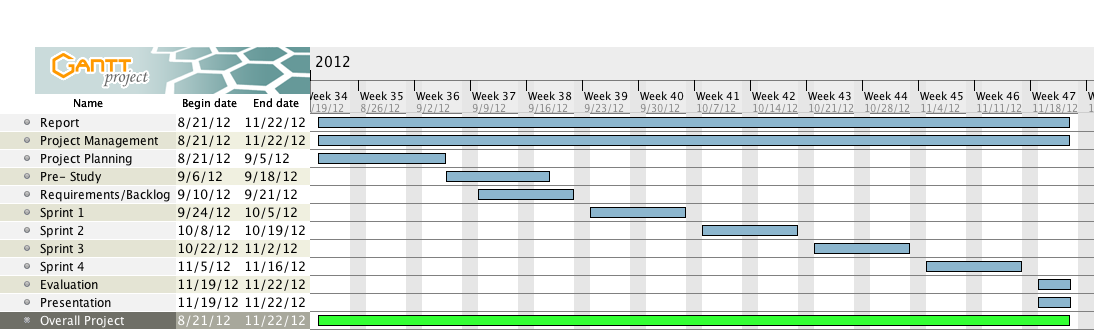
\includegraphics[width=6in]{image/gantt.png}
\caption{Gantt Chart}
\label{figure:gantt}
\end{figure}

\begin{table}
\caption{Work Breakdown Structure}
\centering
\begin{tabular}{ l l l l l }
\hline 
			&				&				&\multicolumn{2}{c}{Hours}		\\
 Task		& From date		&To date			&Est.			&Act.	                \\ 
\hline \\ [-2.0ex]
 The report     			&21/08/2012		&22/11/2012		&300		&         	 \\
 Project Management	&21/08/2012		&22/11/2012		&180		&		\\
 Project Planning		&21/08/2012		&05/09/2012		&100		&		\\
 Lectures				&21/08/2012		&05/09/2012		&40			&		\\	
 Pre- Study			&06/09/2012		&18/09/2012		&80			&		\\
 Backlog				&10/09/2012		&21/09/2012		&60			&		\\
 Architecture			&17/09/2012		&21/09/2012		&40			&		\\
\hline \\ [-2.0ex]
 \bf{Sprint 1}			&\bf{24/09/2012}	&\bf{05/10/2012}	&\bf{130}		&		\\
 Planning				&				&				&20			&		\\
 Design/Implementation	&				&				&90			&		\\
 Testing				&				&				&20			&		\\
\hline \\ [-2.0ex]
 \bf{Sprint 2}			&\bf{08/10/2012}	&\bf{19/10/2012}	&\bf{130}		&		\\
 Planning				&				&				&20			&		\\
 Design/Implementation	&				&				&90			&		\\
 Testing				&				&				&20			&		\\
\hline \\ [-2.0ex]
 \bf{Sprint 3}			&\bf{22/10/2012}	&\bf{02/11/2012}	&\bf{140}		&		\\
 Planning				&				&				&20			&		\\
 Design/Implementation	&				&				&100		&		\\
 Testing				&				&				&20			&		\\
\hline \\ [-2.0ex]
 \bf{Sprint 4}			&\bf{05/11/2012}	&\bf{16/11/2012}	&\bf{140}		&		\\
 Planning				&				&				&20			&		\\
 Design/Implementation	&				&				&100		&		\\
 Testing				&				&				&20			&		\\
\hline \\ [-2.0ex]
 Evaluation			&19/11/2012		&22/11/2012		&30			&		\\
 Presenation			&19/11/2012		&21/11/2012		&30			&		\\
\hline \\ [-2.0ex]
 \bf{Total}			&				&				&\bf{1400}	&		\\
\hline
\end{tabular}
\label{table:wbs}
\end{table}

\section{Project name}
Project name is important project identificator. It should summarize main project goal or functionality. In real project, is often a trademark, or reflects the name of the company.

In this section, we will describe the process of choosing a name for the project. First of all, we made a list of words, that we can use in the project name. These words describe project funcionality or goal.

Words that can be used in project name: master, console, web, text, keyboard.

We used the list of words and brainstorming session on a meeting for compiling a list of project name candidates:

Candidate project names: console 2.0, wonsole, wensole, websole, werminal, interCLI.

After discussion we chose the name \emph{Wonsole}. Project name can be sometimes little confusing, so we added the subtitle: \emph{The new web console for power users.}


\section{Team Structure}
We are a very small development team of just four team members. In typicall software project, there is a lot of different roles, so each of us have to have more roles. We started with creating a list of roles, that we need in the team. Each role represents a responsibility. This person should have overview of the progress on his area of responsibility and control the work done. The work itself is beeing broken down into tasks and on these tasks can work anyone from the team. The roles in our team are listed in the table \ref{table-teamroles}, overview of the roles is in the table \ref{table-rolesoverview}.

\begin{table}
\centering
\begin{tabular}{ l  l }
  \hline
  \textbf{Team member} & \textbf{Roles} \\
  Ivo & Group leader, Customer and Advisor Contact, Scrum Master \\
  Oystein & Test Manager, QA Manager, Weekly Report Manager \\
  Oddvar & GUI Designer, Code Master, Meeting Secretary, Time Keeper \\
  Martin & System Architect, Report Manager \\
  \hline
\end{tabular}
\label{table-rolesoverview}
\caption{Team role overview}
\end{table}


\begin{table}
\begin{tabularx}{\textwidth}{ | l | X | l | }
  \hline
  \textbf{Role} & \textbf{Description} & \textbf{Assignee} \\ 
  \hline
  Team leader & Is responsible for administrative tasks and makes the final decisions. & Ivo \\ 
  \hline
  Scrum Master & Shields the development team from external distractions and enforces the Scrum scheme.  & Ivo \\ 
  \hline
  Customer Contact & Handles communication with the customer. The customer should contact this person regarding general requests, questions and reminders. & Ivo (backup Martin) \\ 
  \hline
  Advisor Contact & Handles communication with the advisor. The advisor should contact this person regarding general requests, questions and reminders.  & Ivo (backup Martin) \\ 
  \hline
  System Architect & Is responsible for the system architecture including distinctions and relations between subsystems and general code design choices. & Martin \\ 
  \hline
  Code Master & Overall responsible for code management and structure. Managing branches in Git repository. & Oddvar  \\ 
  \hline
  GUI Designer & Is responsible for the layout and design of graphical user interfaces. & Oddvar \\ 
  \hline
  Test Manager & Is responsible for testing including unit tests, integration tests and usability tests. & Øystein \\ 
  \hline
  Report Manager & Is responsible for delegating and overseeing work on the project report. & Martin \\ 
  \hline
  Customer Representative & Participates in regular meetings to discuss the progress, project status and future tasks. Represents the customer. & Peder Kongelf \\ 
  \hline
  Customer Technical Advisor & May be consulted about technical aspects of the project. & Stig Lau \\ 
  \hline
  Advisor & Serves as a one-man steering committee for the project. & Meng Zhu \\ 
  \hline
  Meeting Secretary & Is responsible for making sure notes get written and sent after each meeting with the advisor and customer. & Oddvar \\ 
  \hline
  Quality Assurance Manager &  & Øystein \\ 
  \hline
  Weekly Report Writer & Is responsible for finalizing the weekly report(s) for the advisor and customer, and getting these delivered for approval. Also responsible for meeting agendas and their delivery. & Øystein \\ 
  \hline
  Time Keeper & Responsible for making sure that everybody is logging their work, and logging team activities. & Oddvar \\ 
  \hline
\end{tabularx}
\caption{Team role}
\label{table-teamroles}
\end{table}

\section{Quality Assurance}
\subsection{Communication rules}
Communication with the customer is usually done by mail. The customer will contact the assigned customer contact if anything else is not specified. The assigned customer contact is responsible for relaying any information received from the customer to the other group members as soon as possible. The customer contact is also responsible for sending any information from the group to the customer. Any communication from the customer demanding a reply, will be replied to within 8 hours. If any communication is sent from the group to the customer demanding a reply, this reply should be received by the group within 24 hours.

The same rules apply to the communication with the advisor.

\subsection{Internal Routines}
Each group member is responsible for logging all their work hours in the timekeeping system within 22:00 the same day. All group members are also responsible for checking the Skype group conversation within 22:00 Monday to Thursday, to see if any important information is posted there. If important information has to be delivered after this time, it will be sent by mail. All group members are required to check Redmine each day to check if any new task are assigned to that person.

\subsection{Deliverables}
All deliverables, including source code, documents and meeting notes, will be approved by at least two of the group members before it is sent for approval by either the advisor or the customer. All major phase documents must be approved by all the group members before it is relayed to the advisor for approval.

\subsection{Meetings}

\subsubsection{Advisor meetings}
Advisor meetings will occur every Thursday 09:15, unless anything else is specified, so the advisor gets updated on the latest work and progress of the project. The day before the meeting the group sends the advisor an agenda for the meeting and a status report of what is done since the last meeting. This will be sent to the advisor within 14:00 the day before the meeting. If this deadline is not sustained, any needed documents will be printed out and brought to the meeting. This lets the advisor enter the meeting prepared, and improve the efficiency of the meeting. Under the meeting issues regarding the work done, plans for next week and project management will be discussed. If there is a sprint-end-week the demo for this sprint will also be shown. Advisor notes will be written during the meetings, compiled and sent back to the advisor within 12:00 the following day.

\subsubsection{Customer meetings}
Customer meetings will occurs on demand, but usually weekly, and Thursdays 19:15 if there is a sprint-end-week, unless anything else is specified. Meetings will be scheduled at least 48 hours before the meeting starts, and confirmation from the customer should be received at least 24 hours before. An agenda for the meeting and a weekly progress report will be sent to the customer to keep him in the loop of the progress, and get prepared before the meetings. This documentation, including other documents needed for the meeting, will be sent by mail within 24 hours before the meeting. Since the customer is busy during work hours, the meetings are kept after 18:00 on weekdays, and after 12:00 in weekends. They will be kept over Skype, since the customer is located in Oslo. The meetings will be used to get the customer in the loop, clarify uncertainties and redirecting, if the direction of the project taken is not what the customer had in mind. The customer should also be included in the sprint planning meetings to help with use case prioritization. Customer notes will be written during the meetings, compiled and sent back to the customer within 12:00 the following day.

\subsubsection{Internal meetings}
Internal meetings will occur every Monday 12:15, unless anything else is specified. At this time all the group members are open for meetings. During these meetings the plans for the week will be discussed, workload divided and what was done last week. Notes will be taken and documented for later review. The group meet daily on skype to keep everyone up to date on the project progress and what will be done.

\subsubsection{Sprint planning meetings}
Sprint planning meetings will be held in the start of every sprint. Which use cases to handle and complete will be discussed here. The tasks will also be discussed with the customer so the customer can help prioritise the use cases and tell us which tasks they want us to complete first. The selected user stories along with their Work Breakdown Structure will be sent to the customer for approval.

\subsubsection{Sprint demonstration meetings}
Sprint demonstration meetings will be held Thursdays 19:15 in the end of the each sprint, unless anything else is specified. The group and the customer will be attending these meetings. An agenda will be sent to the customer, together with the weekly report and a link to the system, for the customer to test out. The demo will show the system and its new functionality. This lets the customer see the progress, and be able to come with inputs towards how their minds might differ from what has been produced, so the group can get on the right track if that is needed. This lets us make sure that we do not stray too far from the intended system. Since this is a meeting held with the customer the rules from the customer meetings will be held, so customer notes will be written during the meetings, compiled and sent back to the customer.

\subsection{Version Control}
GitHub was selected as the tool for version control in this project. All the relevant work that is produced will be pushed to the repository using git, including all the documents for the report, source code, images, diagrams, and so on. The group members will commit and push their changes on a regular basis, ensuring that the repository is always up to date and available.

\subsection{Document Templates}
The group has created templates for the following documents:

\begin{itemize}
\item Weekly status report
\item Meeting agenda
\item Meeting notes
\end{itemize}

These templates are listed in the appendices.

\chapter{Risk Table}

\begin{table}
\begin{tabularx}{\textwidth}{ | l | X | l | l | }
  \hline
  \textbf{\#} & \textbf{Risk} & \textbf{Probability} & \textbf{Impact} \\ \hline
  1 & Not getting a fifth party member & M & Significant \\ \hline
  2 & Obtrusive health/family/personal issues for team members & L & Significant \\ \hline
  3 & Low morale in team & M & Significant \\ \hline
  4 & Interfering workload from other activities & H & Minor \\ \hline
  5 & Miscommunication with customer & M & Critical \\ \hline
  6 & Changes in customer requirements & M & Significant \\ \hline
  7 & Errors in project plan & M & Significant \\ \hline
  8 & Failure of communication in team & M & Critical \\ \hline
  9 & Failure of time management & H & Critical \\ \hline
 10 & Errors in workload estimation and distribution & H & Critical \\ \hline
 11 & Failure of online storage systems and services & L & Significant \\ \hline
 12 & Failure of personal computers & M & Significant \\ \hline
 13 & Infeasibility of project as a whole & L & Critical \\ \hline
 14 & Inability to find potential users and test subjects & M & Significant \\ \hline
\end{tabularx}
\caption{Risk overview}
\end{table}


\begin{table}
\begin{tabularx}{\textwidth}{ | l | X | }
\hline
\textbf{Risk \#} & 01 \\ \hline
\textbf{Activity} & All \\ \hline
\textbf{Risk Factor} & Not getting a fifth party member \\ \hline
\textbf{Impact} & Significant \\ \hline
\textbf{Consequence} & Increased workload for all remaining party members on all activities \\ \hline
\textbf{Probability} & Medium \\ \hline
\textbf{Countermeasures} & \begin{itemize}
  \item  Contact advisor about the dropped party member, try to get assigned a new member.
  \item Take the missing person into account in planning phase.
\end{itemize}  \\ \hline
\textbf{Deadline} & Intro/Planning (Ultimately in the hands of course staff) \\ \hline
\textbf{Responsible} & Project leader \\ \hline
\end{tabularx}
\caption{Risk 01}
\end{table}

\medskip

\begin{table}
\begin{tabularx}{\textwidth}{ | l | X | }
\hline
\textbf{Risk \#} & 02 \\ \hline
\textbf{Activity} & All \\ \hline
\textbf{Risk Factor} & Obtrusive health/family/personal issues for team members \\ \hline
\textbf{Impact} & Significant \\ \hline
\textbf{Consequence} & Increased workload for all remaining party members on all activities \\ \hline
\textbf{Probability} & Low  \\ \hline
\textbf{Countermeasures} & \begin{itemize}
  \item Implement buffers in project plan.
  \item Team members should make their work resumable by another member.
\end{itemize}  \\ \hline
\textbf{Deadline} &  None \\ \hline
\textbf{Responsible} & Project leader \\ \hline
\end{tabularx}
\caption{Risk 02}
\end{table}

\medskip

\begin{table}
\begin{tabularx}{\textwidth}{ | l | X | }
\hline
\textbf{Risk \#} & 03 \\ \hline
\textbf{Activity} & All \\ \hline
\textbf{Risk Factor} & Low morale in team \\ \hline
\textbf{Impact} & Significant \\ \hline
\textbf{Consequence} & Decreased overall project quality \\ \hline
\textbf{Probability} & Medium  \\ \hline
\textbf{Countermeasures} & \begin{itemize}
  \item Frequent contact between team members
  \item Avoid team members overworking
  \item Focus on general team dynamics advice from advisor
\end{itemize}  \\ \hline
\textbf{Deadline} &  None \\ \hline
\textbf{Responsible} & Project leader \\ \hline
\end{tabularx}
\caption{Risk 03}
\end{table}

\medskip

\begin{table}
\begin{tabularx}{\textwidth}{ | l | X | }
\hline
\textbf{Risk \#} & 04 \\ \hline
\textbf{Activity} & All \\ \hline
\textbf{Risk Factor} & Interfering workload from other activities \\ \hline
\textbf{Impact} & Low \\ \hline
\textbf{Consequence} & Work on the project is shifted in time, space and responsibility \\ \hline
\textbf{Probability} & Very High \\ \hline
\textbf{Countermeasures} & \begin{itemize}
  \item Plan ahead with respect to existing schedules
  \item Inform the group of other activities
\end{itemize}  \\ \hline
\textbf{Deadline} &  None \\ \hline
\textbf{Responsible} & Project leader \\ \hline
\end{tabularx}
\caption{Risk 04}
\end{table}

\medskip

\begin{table}
\begin{tabularx}{\textwidth}{ | l | X | }
\hline
\textbf{Risk \#} & 05 \\ \hline
\textbf{Activity} & All \\ \hline
\textbf{Risk Factor} & Miscommunication with customer \\ \hline
\textbf{Impact} & Critical \\ \hline

\textbf{Consequence} & -The project is not developed as the customer wants it
-Work has to be done over \\ \hline
\textbf{Probability} & Very High \\ \hline
\textbf{Countermeasures} & \begin{itemize}
  \item Weekly customer meetings
  \item Share as much information as possible with customer at all stages
\end{itemize}  \\ \hline
\textbf{Deadline} &  None \\ \hline
\textbf{Responsible} & Customer Contact \\ \hline
\end{tabularx}
\caption{Risk 05}
\end{table}

\medskip

\begin{table}
\begin{tabularx}{\textwidth}{ | l | X | }
\hline
\textbf{Risk \#} & 06 \\ \hline
\textbf{Activity} & Planning, Requirements, Implementation \\ \hline
\textbf{Risk Factor} & Changes in customer requirements \\ \hline
\textbf{Impact} & Significant \\ \hline
\textbf{Consequence} & Work has to be done over  \\ \hline
\textbf{Probability} & Medium \\ \hline
\textbf{Countermeasures} & \begin{itemize}
  \item Design the prototype with possible modifications in mind.
  \item Try to get information on possible changes from the customer.
\end{itemize}  \\ \hline
\textbf{Deadline} &  None \\ \hline
\textbf{Responsible} & Customer Contact \\ \hline
\end{tabularx}
\caption{Risk 06}
\end{table}

\medskip

\begin{table}
\begin{tabularx}{\textwidth}{ | l | X | }
\hline
\textbf{Risk \#} & 07 \\ \hline
\textbf{Activity} & Implementation \\ \hline
\textbf{Risk Factor} & Errors in project plan \\ \hline
\textbf{Impact} & Significant \\ \hline
\textbf{Consequence} & Work on the plan and implementation have to be redone  \\ \hline
\textbf{Probability} & Medium \\ \hline
\textbf{Countermeasures} & \begin{itemize}
  \item Review the project plan frequently for consistency
  \item Share plan with customer
\end{itemize}  \\ \hline
\textbf{Deadline} &  Planning \\ \hline
\textbf{Responsible} & Project Leader \\ \hline
\end{tabularx}
\caption{Risk 07}
\end{table}

\medskip

\begin{table}
\begin{tabularx}{\textwidth}{ | l | X | }
\hline
\textbf{Risk \#} & 08 \\ \hline
\textbf{Activity} & All \\ \hline
\textbf{Risk Factor} & Failure of communication in team \\ \hline
\textbf{Impact} & Critical \\ \hline
\textbf{Consequence} & Failure of unification of the work, uneven workloads, decreased project quality  \\ \hline
\textbf{Probability} & Medium \\ \hline
\textbf{Countermeasures} & \begin{itemize}
  \item Frequent internal meetings
  \item Sharing of work internally
\end{itemize}  \\ \hline
\textbf{Deadline} &  None \\ \hline
\textbf{Responsible} & Project Leader \\ \hline
\end{tabularx}
\caption{Risk 08}
\end{table}

\medskip

\begin{table}
\begin{tabularx}{\textwidth}{ | l | X | }
\hline
\textbf{Risk \#} & 09 \\ \hline
\textbf{Activity} & All \\ \hline
\textbf{Risk Factor} & Failure of time management \\ \hline
\textbf{Impact} & Critical \\ \hline
\textbf{Consequence} & Parts of project are rushed or not finished in time \\ \hline
\textbf{Probability} & High \\ \hline
\textbf{Countermeasures} & \begin{itemize}
  \item Put in as much work as possible as early as possible
  \item Implement buffers in project plan
\end{itemize}  \\ \hline
\textbf{Deadline} &  None \\ \hline
\textbf{Responsible} & Project Leader \\ \hline
\end{tabularx}
\caption{Risk 09}
\end{table}

\medskip

\begin{table}
\begin{tabularx}{\textwidth}{ | l | X | }
\hline
\textbf{Risk \#} & 10 \\ \hline
\textbf{Activity} & All \\ \hline
\textbf{Risk Factor} & Errors in workload estimation and distribution \\ \hline
\textbf{Impact} & Critical \\ \hline
\textbf{Consequence} & Uneven workloads, rushed or unfinished parts of project \\ \hline
\textbf{Probability} & High \\ \hline
\textbf{Countermeasures} & \begin{itemize}
  \item Implement buffers in project plan
  \item Avoid relying too much on rigid plans
  \item Allow for redistribution of work when necessary
\end{itemize}  \\ \hline
\textbf{Deadline} &  Planning \\ \hline
\textbf{Responsible} & Project Leader \\ \hline
\end{tabularx}
\caption{Risk 10}
\end{table}

\medskip

\begin{table}
\begin{tabularx}{\textwidth}{ | l | X | }
\hline
\textbf{Risk \#} & 11 \\ \hline
\textbf{Activity} & All \\ \hline
\textbf{Risk Factor} & Failure of online storage systems and services \\ \hline
\textbf{Impact} & Critical \\ \hline
\textbf{Consequence} & Work is lost and has to be recreated \\ \hline
\textbf{Probability} & Low \\ \hline
\textbf{Countermeasures} & \begin{itemize}
  \item Local backups of data
  \item Know of alternative systems in case of failure
\end{itemize}  \\ \hline
\textbf{Deadline} &  None \\ \hline
\textbf{Responsible} & Project Leader \\ \hline
\end{tabularx}
\caption{Risk 11}
\end{table}

\medskip

\begin{table}
\begin{tabularx}{\textwidth}{ | l | X | }
\hline
\textbf{Risk \#} & 12 \\ \hline
\textbf{Activity} & All \\ \hline
\textbf{Risk Factor} & Failure of personal computers \\ \hline
\textbf{Impact} & Significant \\ \hline
\textbf{Consequence} & Work may be lost, decreased productivity of team member \\ \hline
\textbf{Probability} & Medium \\ \hline
\textbf{Countermeasures} & \begin{itemize}
  \item Use primarily online storage systems and keep online backups of everything else
  \item Use university computers if necessary
\end{itemize}  \\ \hline
\textbf{Deadline} &  None \\ \hline
\textbf{Responsible} & Individual \\ \hline
\end{tabularx}
\caption{Risk 12}
\end{table}

\medskip

\begin{table}
\begin{tabularx}{\textwidth}{ | l | X | }
\hline
\textbf{Risk \#} & 13 \\ \hline
\textbf{Activity} & All \\ \hline
\textbf{Risk Factor} & Infeasibility of project as a whole \\ \hline
\textbf{Impact} & Critical \\ \hline
\textbf{Consequence} & The concept is not a solution to the problem and the prototype is destined to be a failure \\ \hline
\textbf{Probability} & Very Low \\ \hline
\textbf{Countermeasures} & \begin{itemize}
  \item Extensive preliminary study to uncover this as early as possible
\end{itemize}  \\ \hline
\textbf{Deadline} & Feasibility study \\ \hline
\textbf{Responsible} & Project Leader \\ \hline
\end{tabularx}
\caption{Risk 13}
\end{table}

\medskip

\begin{table}
\begin{tabularx}{\textwidth}{ | l | X | }
\hline
\textbf{Risk \#} & 14 \\ \hline
\textbf{Activity} & Planning \\ \hline
\textbf{Risk Factor} & Inability to find potential users and test subjects \\ \hline
\textbf{Impact} & Significant \\ \hline
\textbf{Consequence} & Requirements engineering and prototype testing will be sub-standard unable to provide adequate answers \\ \hline
\textbf{Probability} & Medium \\ \hline
\textbf{Countermeasures} & \begin{itemize}
  \item Try to get information on potential users from customer
  \item Begin contacting potential users and testers early
\end{itemize}  \\ \hline
\textbf{Deadline} & Testing \\ \hline
\textbf{Responsible} & Project Leader \\ \hline
\end{tabularx}
\caption{Risk 14}
\end{table}



\section{Lectures}
\section{Issues}


\section{Domain choosing}
\begin{comment}
Domain ideas:
project management tool (ehm. redmine)
warehouse
airport / travel agency
cash registers (not interesting)
bank
school information system (boring)
time management system (aka calendar)
facebook console (unreal)
mail interface (gmail is too good, not useful)
photo gallery (limited)
music library (limited)
physician system (treatments, prescriptions, add person)
tax form (boring)
Building management (boring)
Library

(ehm. redmine) 
warehouse 1
1
bank 3 3
(aka calendar) 2
(treatments, prescriptions, add person) 1
Library 2 2 3

Ivo	Martin	Oddvar	Oystein	Total
project management tool	3		2		5
warehouse			1		1
airport / travel agency		1			1
bank		3		3	6
time management system	2				2
physician system	1			1	2
Library		2	3	2	7




Top3:
library
authors, books(location, state), book management, employees, user management, order new books, 

bank
accounts, transfer money, deposits, loans, customer management, employees

project management
projects, issues, work done on issues, workers, sprints, reports, 

interesting	simple to understand	complex enough	ease workflow	existence of power user	total
library	2	3	1	2	Y	8
bank	2	3	2	2	Y	9
project management	1	2	3	2	Y	8



project management
+ usefulness
+ field of study
- boring

library
+ libraries in campus, employees
- simple

bank
- unknown ground


library	project management	bank
martin	3	2	1
oddvar	3	2	1
ivo	2	3	1
oystein	3	1	2
total	11	8	5



Criteria:
Interesting and simple enough for test subjects to understand. something they meet in everyday life
Complicated enough to demonstrate the problem.
Console has to be useful in the domain, ease the workflow
Object oriented design
Existence of power user, that will use the console

Customer ideas:
car models
finn.no
health sector
human resources (people, how they are related, symptoms, how much money and what they own - advanced domain graph). 
contact lists (peder)


write these things to the report


Future:
batch operations
undo the commands
save command for object attribute editing
what about object operations?
transaction support
\end{comment}

\chapter{Preliminary Study}

\minitoc

\subsubsection{Purpose}

\clearpage

\section{Concept}

\section{Constraints}
\subsection{Time}
The project must be completed within a timeframe of 13.6 weeks. The guideline is 24.3 work hours per person, per week. 
\subsection{Knowledge about the problem}
Our problem is not well-explored and the customer cannot give us exact requirements. Thus, this is as much a research project as it is a software development project.

\section{Feasibility study}

\section{Similar solutions}

\subsection{Counter-Strike}

\begin{figure}
\centering
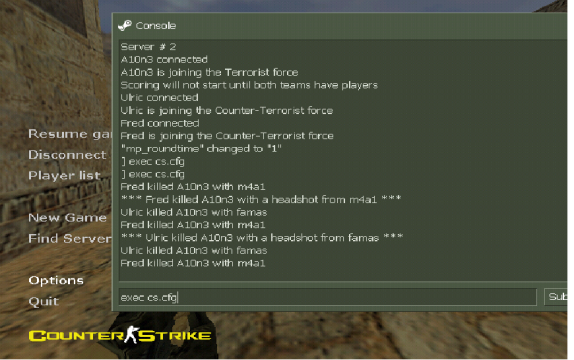
\includegraphics[width = 0.8\textwidth]{image/counterstrike.png}
\caption{Counter-Strike console}
\label{image-counterstrike}
\end{figure}

This game features a console that offers a wide variety of commands, including:
- Changing the game options
- Altering the game world
- Player actions and cheats
- Multiplayer communication and administration
Example screenshot is on \ref{image-counterstrike}.

In a game, this functionality eases development and debugging, as well as increasing the moddability and long-term value for players. Similar consoles also exist in other games, such as Carmageddon TDR 2000.

\subsection{Blender}

\begin{figure}
\centering
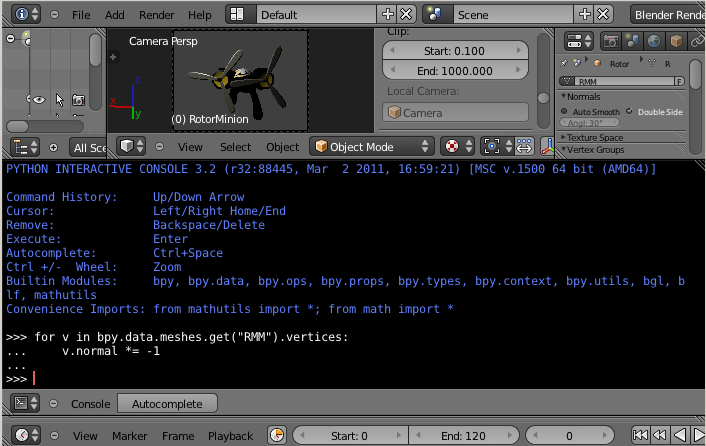
\includegraphics[width = 0.8\textwidth]{image/blender.png}
\caption{Blender console}
\label{image-blender}
\end{figure}

This 3D modelling software features a Python console with access to the model data, animation data, etc. It can be used to perform operations that are not directly supported in the user interface. It is also common to extend the program using custom Python scripts. 

Similar solutions also exist in other creative tools, including a Python console in GIMP and Nyquist prompt in Audacity.

Example screenshot is on \ref{image-blender}.

\subsection{Firefox}

\begin{figure}
\centering
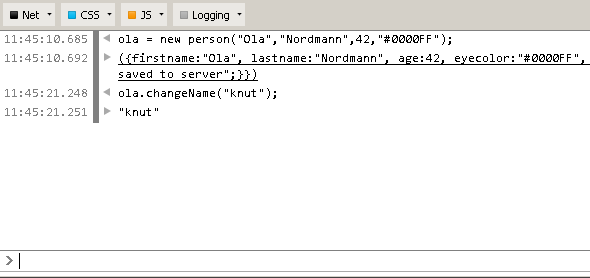
\includegraphics[width = 0.8\textwidth]{image/firefox.png}
\caption{Firefox console}
\label{image-firefox}
\end{figure}

This web browser features a Web Console where it is possible to execute JavaScript commands with access to the objects on the current page. This is useful for web development and debugging. Similar features also exist in a few other browsers, such as Google Chrome.

Example screenshot is on \ref{image-blender}.

\subsection{try.mongodb.org}

\begin{figure}
\centering
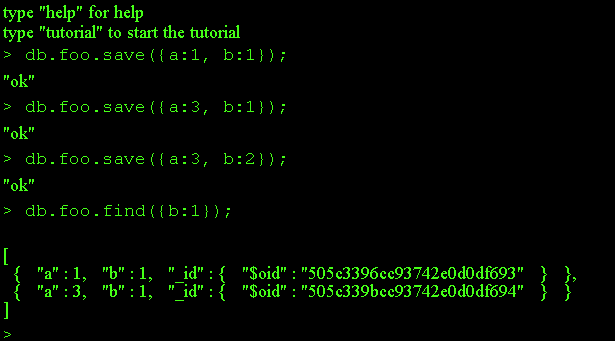
\includegraphics[width = 0.8\textwidth]{image/mongodb.png}
\caption{MongoDB console}
\label{image-mongo}
\end{figure}

This database website features a console where the user can execute commands on a dummy database. It is an educational tool for people who don't want to invest too much time in it. Comparable consoles also exist to allow the user to execute arbitrary queries in database administration tools such as PHPMyAdmin.

Example screenshot is on \ref{image-mongo}.

\subsection{web-console.org}

\begin{figure}
\centering
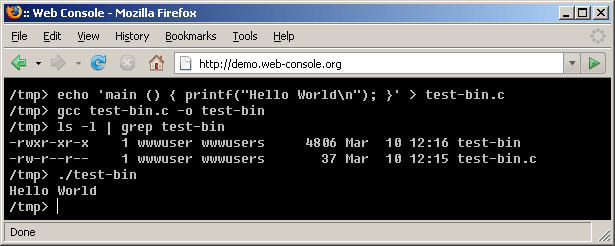
\includegraphics[width = 0.8\textwidth]{image/webconsole.png}
\caption{Web-console}
\label{image-webconsole}
\end{figure}

This project provides shell access to a server through the browser window over HTTP.

It supports real time communication, and is intended to be used for server administration purposes.

Example screenshot is on \ref{image-webconsole}.

\subsection{Conclusion}

This is by no means an exhaustive list, but it serves to illustrate that consoles are still applicable for purposes including software development, debugging, learning, extendability and where there is a high demand for flexibility.



\section{Version control}
\subsection{git}

\section{Development language and technologies}
\subsection{Colaboration}

\subsubsection{Redmine}

\begin{wrapfigure}{r}{.25\textwidth}
\vspace{-30pt}
\centering

\includegraphics[width = .30\textwidth]{image/redmine-logo.pdf}
\end{wrapfigure}

Redmine is online project management tool. It is an open source, cross-platform application. If offers role based access control, issue tracking system, Gantt chart display, browsing source code saved on git. We use this application to plan project, create, assign and log issues. It can be also used as alternative source code browser with its own automatically replicated copy of github repository. Information stored in the system are very important, so we did set up automatic backup of database to git.
\footnote{http://www.redmine.org/projects/redmine/wiki}

\subsubsection{Google Calendar}

\begin{wrapfigure}{r}{.25\textwidth}
\vspace{-30pt}
\centering
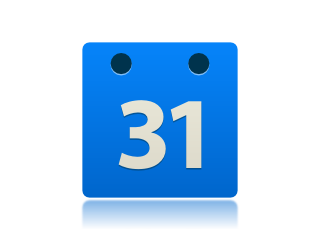
\includegraphics[width = .20\textwidth]{image/calendar-logo.png}
\end{wrapfigure}

Google Calendar is online time management tool, which enables users to create events in shared calendars. It is also possible to invite people to attend an event. We use it for planning the meetings, and put in important lectures and deadlines. Shared calendar is administered by team members.
\footnote{https://www.google.com/calendar}

Our group Google Calendar is available on page:
https://www.google.com/calendar/embed?src=6j792hr87jahd4vpnj636h1080%40group.calendar.google.com

\subsubsection{Google Groups}

\begin{wrapfigure}{r}{.25\textwidth}
\vspace{-30pt}
\centering

\includegraphics[width = .20\textwidth]{image/groups-logo.png}
\end{wrapfigure}

Google Groups is online communication tool. It offers group management and communication through web interface and email. We use it as a mailing list tool. Contact person publishes important news and information. Meeting dates and notes are distributed to all members of group. Customer and advisor can send emails directly to group email address, so that if contact person is not available at the moment, anyone from group can answer.

Our Google Group mailing list address is: ntnu-netlight-project@googlegroups.com
\footnote{https://groups.google.com/googlegroups/overview.html}

\subsubsection{Google Drive}

\begin{wrapfigure}{r}{.25\textwidth}
\vspace{-30pt}
\centering

\includegraphics[width = .20\textwidth]{image/drive-logo.jpg}
\end{wrapfigure}

A file storage and synchronization service. Google Drive is the home of Google Docs, which is a set of applications such as document editing, spreadsheet, powerpoint, etc. We use these applications to easy share all documents between all the members of our project. It lets us edit and work with the same documents separately at the same time, and keeps a safe backup in the Google Cloud of our files if some computers where to break down.
\footnote{http://en.wikipedia.org/wiki/Google\_Drive}


\subsubsection{Skype}

\begin{wrapfigure}{r}{.25\textwidth}
\vspace{-30pt}
\centering

\includegraphics[width = .20\textwidth]{image/skype-logo.png}
\end{wrapfigure}

A free P2P/client-server communication program. It lets the users communicate with each other through voice, video, instant messaging and file transferring. The users needs a Skype account to reach other Skype users. This program is a VoIP service which lets us communicate without any extra cost if connected to a network. We mainly use Skype for discussions when the group is not gathered, this also gives us a transcript of what was discussed.
\footnote{http://en.wikipedia.org/wiki/Skype}

\subsubsection{GitHub}

\begin{wrapfigure}{r}{.25\textwidth}
\vspace{-30pt}
\centering

\includegraphics[width = .20\textwidth]{image/github-logo.png}
\end{wrapfigure}

Web-based hosting service for software development. It uses the Git revision control system. Git focus on speed, and gives the user full revision tracking. GitHub uses this to present different functionalities to the users, such as setting up repositories, forking repositories, writing wikis and setting up web pages for the repositories.
\footnote{http://en.wikipedia.org/wiki/GitHub}
\footnote{http://en.wikipedia.org/wiki/Git\_\(software\)}

\subsubsection{LaTeX}

\begin{wrapfigure}{r}{.25\textwidth}
\vspace{-30pt}
\centering

\includegraphics[width = .20\textwidth]{image/latex-logo.png}
\end{wrapfigure}

LaTex is a document markup language that uses the TeX typesetting program. The main focus of LaTex is to make authors able to focus on the content of what they are writing without worrying about its visual presentation. It is mainly used to transform XML- based documents to PDFs. LaTex is widely used in academia, to produce scientific reports, etc.

\subsection{Database}
For the system we need some kind of persistent storage, a database which all the clients can talk to to get the latest data in the system and to synchronise data from different clients. This database will be placed on a central server which all the clients can communicate with. For the database we are left with a decision between traditional SQL database or a socalled NoSQL database. The differences are explained below.

\subsubsection*{NoSQL}
NoSQL arose from the need to store large amount of data that do not necessarily follow the same schema, or share all the same attributes. The main characteristic of NoSQL databases is their schema- less structure. They also differ from SQL by generally not using a structured query language for data manipulation. They are easy to replicate and they offer simple APIs for the clients to communicate with. They are heavily customised for web- applications, and have gained much popularity in the modern web era. Most NoSQL databases focus on quick replies to requests, as the queries operation is by far the most common in a typical web- application. Because they typically are distributed, NoSQL databases are able to store enormous amounts of data, and they are often used within "Big Data"(explanation) applications like Hadoop(reference), which recently has become a very popular subject within the computer science community. BASE(explanation) instead of ACID. 


\subsubsection*{SQL}
The traditional SQL databases is by far the most common way of storing data in the world today. They store data in columns and tables, and add relationships between these tables. As a result they are referred to as relational databases. They focus on query optimisation techniques and most of them use some kind of structured query language. Typically supports 4 basic operations which is select, update, delete and insert. SQL databases are schema defined and follows the ACID principles(Need explanation somehow)
\newline

\subsubsection{Database Alternatives}
Below, some of the database implementation available to us are discussed. Both NoSQL and traditional SQL options are introduced.

\subsubsection*{MongoDB}
MongoDB is a large scale, high availability, robust system. It is a NoSQL system, so instead of storing the data in tables as you would in MySQL, the data is stored in a document based fashion through for instance JSON with dynamic schemas. This makes the DB easier scalable horizontally. But the mongoDB still possesses the some of the great properties from relational databases, such as indexes, dynamic queries and updates. With mongoDB it is easy to map objects to programming language data types, which makes the DB easy to work with. The embedded documents and arrays makes the join operations less importance, which result in the ability to make reads and writes faster. JavaScripts can also be included in the queries. This makes mongoDB an efficient and high speed data base for storing objects and fetching to a system. MongoDB also has its own access console, where you can use scripting with Javascript language. \cite{mongodb-intro}

\subsubsection*{CouchDB}
CouchDB stores the data in JSON documents(NoSQL) object-oriented, which can be accessed through HTTP. The data documents can be transformed and data fetched with JavaScript. CouchDB has a lot of built in features which makes web development with CouchDB easier. It scales well through replication and is a consistent system, where CouchDB prioritises the data of the user. CouchDB is multiversion concurrency control based, this is good for intense versioning, offline databases which resync later and master to master replication. The interface to the database is REST based, which is a useful feature when you are developing a web- application.
\cite{couchdb-about, couchdb-technical}

\subsubsection*{MySQL}
MySQL is the most popular database in the world of open databases. This is because of its high performance, reliability and ease of use, and should therefore be considered when the question comes to which database system to use. In opposition of the two database systems described above, MySQL is a relational database. This makes it more troublesome to work, with when it comes to JavaScript, than the other two. It is not as well integrated with JSON and will need parsing to be working with the clients. This alone is a hard negative towards MySQL.
\cite{mysql-about}


\subsubsection{Conclusion}
We decided to go for NoSQL in this project. We are working in a web domain, which NoSQL databases were designed for. While developing the console we will be working closely with JavaScript objects, and try to find ways of exposing these to the users. JavaScript objects are easily converted to JSON, the format used to store data in document NoSQL databases like MongoDB and CouchDB.  As we only have the need to store the actual objects and a limited amount of relations between them, using NoSQL will ease our work considerably, and allow us to do things which would not be possible with a regular SQL database. NoSQL imposes far less restrictions on how you store your data than traditional SQL does. As long as the data is represented in JSON, you can store pretty much store anything you like, even within the same database. This will give us great flexibility when it comes to adding information to specific objects, and also means that objects of the same type can contain different attributes without us needing to create a new schema or change anything in the database. It also gives the user great flexibility in the sense that they can add any information they would like to the different objects, and we the developers don't have to plan for it at all, the database does all this for us. As a result, instead of explicitly adding functionality, we can add restrictions to allow the user to add functionality within a certain scope.

The fact that the customer suggested to us that we could use a NoSQL database, also tiped the scale in direction of the NoSQL alternatives. 
\newline
\newline
Relational databases is the traditional way to deploy databases and they are in widespread use. In many situations they are extremely useful. However relational databases requires you to model your data up front, before you save anything to the database. Failing to comply with these restrictions will lead to failure, and it is sometimes difficult to create this kind of model that actually fits real world data. Even though objects may share common attributes, there are bound to be some attributes that are different. This is difficult to plan for in advance, and its the main reason we will not be using a SQL database for this project.
\newline
\newline
For the database, we originally chose to use MongoDB as our NoSQL database. This was due to the fact that it was better documented and seemed better suited for the system as we originally planned it. Some of the features CouchDB offered wasn't thought of as necessary for the project at the time. During the implementation process we however came to the conclusion that CouchDb actually was a better fit. This was mostly due to its ability to act as an standalone system on a server without the need for other supporting server technologies like Node.js or ASP.NET. Also, the fact that it automaticly creates a RESTful API to access the database turned out to save us a lot of time. Its comprehensive versioning control system, which we deemed unnecessary at first, actually turned out to be a great resource. As a result of these discoveries we changed to CouchDb during the third sprint.


\subsection{Backend}
\subsubsection*{Node.js}
Node.js is a platform designed for server side applications. It is written in JavaScript using Google Chrome's JavaScript runtime called V8. The same runtime is used by the MongoDB database engine, so it shares some of its properties. It can be used for building fast and scalable network applications. Also it is very lightweight and efficient \cite{nodejs-about}.

\subsubsection*{ASP.NET}
ASP.NET is a part of the .NET Framework used for creating web applications and services. The framework is language independent, so you can use any language that .NET offers. It also allows programmers to use similar approach in web applications as in desktop applications. On the other hand is not as lightweight as Node.js \cite{aspnet-about}.

\subsubsection*{PHP}
PHP is a acronym for Hypertext Preprocessor. It is a serverside programming language mainly used for web applications. PHP is easy to use and supports a lot of modules, platforms and database systems. One of the main disadvantages is, that is not as effective for web applications, because it is interpreted and doesnt keep application context \cite{php-whatis}.

\subsubsection*{Ruby on Rails}
Ruby on Rails is a web application Framework using the MVC, Model View Controller model. It is a Ruby language module for building dynamic web applications. This framework also offers variety of modules, which can extend functionality or simplify tasks. The code is run the same way as Node.js and PHP, they are all interpreted, but Ruby on Rails is more difficult to install \cite{ror-about}


\subsection{Client-side web application technologies}
Our main focus will be on the client part of the application, since this is the experimental part of our system, and it is this part that is visible to the user through the web browser. It is therefore important to choose a suitable technology for this.

\subsubsection{Adobe Flash}

\begin{wrapfigure}{r}{.15\textwidth}
\vspace{-30pt}
\centering

\includegraphics[width = .10\textwidth]{image/flash-logo.png}
\end{wrapfigure}


A multimedia platform currently owned by Adobe. Is currently the industry standard for multimedia web applications. It excels at animation and 2D games, but its strong points are not likely to be useful in our project. A separate JavaScript is required to perform communication with a server and the development tools are costly.

\subsubsection{Microsoft Silverlight}

\begin{wrapfigure}{r}{.15\textwidth}
\vspace{-47pt}
\centering

\includegraphics[width=.10\textwidth]{image/silverlight-logo.jpg}
\end{wrapfigure}

A rich media application framework developed by Microsoft. Useful for multimedia applications, but likely not beneficial for our project.

\subsubsection{Java Applets}

\begin{wrapfigure}{r}{.15\textwidth}
\vspace{-30pt}
\centering

\includegraphics[width=.14\textwidth]{image/java-logo.jpg}
\end{wrapfigure}

A technology that allows a Java AWT/Swing application to be displayed in a browser, backed by a Java Virtual Machine. Has excellent performance compared to other popular client side browser technologies. A signed applet can also communicate with a server using traditional sockets. It is possible to embed a scripting engine(for instance JavaScript). However, development effort may prove to become excessively heavy.

\subsubsection{JavaScript}

\begin{wrapfigure}{r}{.15\textwidth}
\vspace{-20pt}
\centering

\includegraphics[width=.14\textwidth]{image/javascript-logo.png}
\end{wrapfigure}


JavaScript is a scripting language supported by all popular web browsers. Has extensive frameworks built around it and allows for rapid development. It is also possible to let the user write commands using JavaScript directly.

\subsubsection{Conclusion}
As a team, we have extensive experience with Java, and less with the other technologies. However, we all have at least some experience with JavaScript, and we believe that it is the better choice for this project: The DSL can be implemented by allowing the user to perform operations on the JavaScript objects using (a subset of) the JavaScript language itself. There are also excellent tools for transfer and storage of JavaScript objects. Furthermore, communication between JavaScript and HTML elements is easily achieved.

\subsubsection{JavaScript Related technologies}

\textbf{jQuery}\\*
A JavaScript library that simplifies how to use JavaScript to interact with the webpage, notably selection of Document Object Model elements.\\*
\\*
\textbf{MooTools}\\*
A JavaScript framework that, notably, enhances the Document Object Model and JavaScript's object oriented programming model.\\
\\*
\textbf{Dojo}\\*
A JavaScript toolkit offering asynchronous communication, a packaging system and systems for data storage. Intended to ease rapid JavaScript web development.\\*
\\*
\textbf{HTML5}\\*
A revision of the HTML standard currently still in development. Notably, it supplies support for multimedia and more advanced user interface elements. Is commonly used in conjunction with JavaScript.\\*
\\*
\textbf{CSS}\\*
Cascading Style Sheets, used to specify a consistent look and feel to a series of HTML documents.\\*


\subsection{Synchronization Technologies}
We will be adding a library for bi-directional real time communications between the server and the client, to easily detect changes in the objects on both sides and to replicate these changes to the other side lightning fast. This functionality will ensure data consistency between the client and server side. To make these updates fast and to avoid extra work in creating this functionality ourselves, we will employ an external library to get the work done.

\subsubsection{Pusher}

\begin{wrapfigure}{r}{.2\textwidth}
\centering

\includegraphics[width=.19\textwidth]{image/pusher-logo.jpg}
\end{wrapfigure}

Pusher is a cloud based system which offers a hosted API. It relies on the use of HTML5 WebSockets, which provides bi-directional communication over a TCP channel. It is a widely used solution which is well documented, and it support for a lot of libraries for both the server and client side. The web-site offers tutorials and extensive documentation on the most popular libraries. 

\begin{figure}
\centering
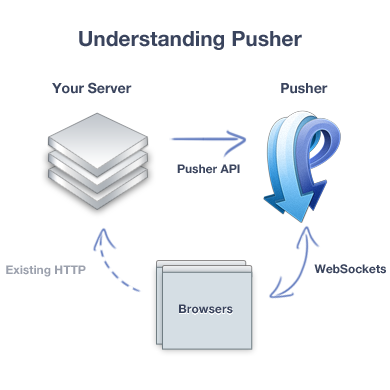
\includegraphics[width=3in]{image/pusher-explained.png}
\caption{Pusher Explained}
\end{figure}


Pusher creates channels that can be both listened and published to. If multiple devices are connected to the same channel, they will receive any messages sent to the channel almost simultaneously. Pusher offers a free account(an account is needed to use the system) which offers all the basic functionality we need, with up to 20 connections and 3 million messages per month

\subsubsection{PubNub}

\begin{wrapfigure}{r}{.2\textwidth}
\centering

\includegraphics[width=.19\textwidth]{image/pubnub-logo.png}
\end{wrapfigure}

Like Pusher, PubNub is a push service hosted in the cloud. It is written entirely in C, which gives it extremely fast performance and enables it to push over 1 million messages a second. It offers great documentation and support for the most popular libraries on both the client and server side and its in widespread use.

Like Pusher it relies on channels for communication which you can subscribe and publish to, and in essence the two solutions work in the same intuitive way. PubNub offers a free account with 1 million messages a month and up to 100 connections.

\subsubsection{Other Technologies}
We considered other similar alternatives as well, like Socket.io, Vert.x and Akka. But they either lacked support for the technologies we have chosen for the system, or lacked the extensive documentation and widespread use that Pusher and PubNub provides. We were also left with the impression that we would spend more time implementing these services than if we opted for either Pusher or PubNub.

\subsubsection{Conclusion}
Pusher and PubNub are both great systems that are widely used and they both offer extensive documentation. They cover the specific functionality we need for this project, which is to replicate the changes on both the client and server side. They both offer free accounts with more than enough connections and messages each month to cover our needs. So this decision will come down to our gut feeling. 

As none of the developers have any experience in using either system, the most important factor for this decision is that the system is well documented and easy to use. During research it became apparent that PubNub is the most widespread solution as of today. If we run into any problems implementing and using the system, it is likely someone has already provided a solution for it. So the decision ultimately fell on using PubNub.


\subsection{Markup Languages}
When communicating between the client and the server we need a data exchange format to represent objects and actions. The format has to be able to serialize and deserialize them on sending and receiving. The two alternatives most commonly in use today for solving this problem is XML (Extensive Markup Language) and JSON (JavaScript Object Notation).

\subsubsection{XML}
In widespread use in a lot of areas as of today and boasts great support and documentation. Originally meant to be a document markup language, but has over the years been used as a data representation language as well. It is suited to describe complex objects and documents, and it is easy to extend. Generally thought of as the more secure option of the two.

\subsubsection{JSON}
As the name suggest JSON is serialized JavaScript objects, well suited for web development, and very fast. JSON is easy for JavaScript to parse(we will be using JavaScript on both server and client), and the language has built in support for serializing and evaluating JSON data. Its small, simple, and easy to use. JSON is especially good at representing programming-language objects. It has gained a great deal of popularity in recent years, and it is well documented.

\subsubsection{Conclusion}
Both languages is well supported in almost all web related libraries, and they are both extensively documented. As security is not a main concern of this project, the fact that XML is more secure will not influence the decision

JSON will be used for this project. It covers the functionality we need, and it is generally thought of as the easier language to use. It is perfectly suited for web- development and JavaScript, which is the domain of this project. In addition the developers have more experience in using JSON than XML.

\subsection{Google Drive}

\section{Development Methodology}
\subsection{Agile vs Waterfall}
The waterfall method focus on planning the future in detail. It follows the principle of “Big Design Up Front”. It relies on the fact that you are able to report exactly what features that are going to be implemented and tasks are planned for the entire length of the project. It forces you to specify all the requirements early in the development, when you actually know the least about the project and the problems that are to be solved. The rationale behind this is that time spent early on making sure requirements and design are correct saves you much time and effort later. A development team using the waterfall method will only consider to implement the most valuable changes, as changes in this process are time consuming and often requires that completed work is started over. The method places a lot of emphasis on documentation. 

Agile methods, as opposed to the predictive methods, are designed to plan for changes in the requirements and features of a project. It emphasises on working code as primary measure of progress, instead of extensive documentation of for example the requirements. Agile methods consists of iterative and incremental steps in the development process, where requirements and solutions evolve through the course of the project. Requirements are bound to change, either because the customer didn't understand the problem in the beginning or because they would like to add new features. Agile methods facilitates the ability to accommodate these changes. Most agile methods includes delivering a working product in incremental stages, and gives the customer something to relate to during the developments process.

The CHAOS Manifesto is a survey published by the Standish Group each year and it measures the success of IT- projects. It divides the projects into 3 groups; Success, meaning it completed on time and budget, with all features and functions as specified. Challenged, meaning it  completed, but was over cost, over time, and/or lacking all of the features and functions that were originally specified. Failed, meaning the project was abandoned or cancelled at some point and thus became a total loss.

\begin{figure}
\centering
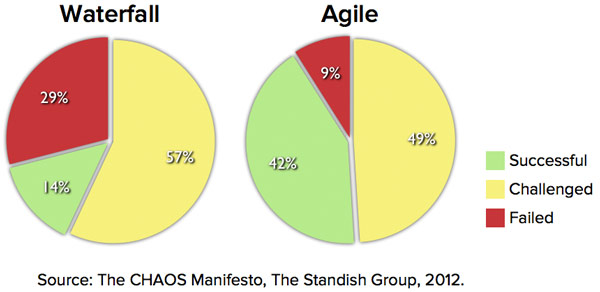
\includegraphics[width=3in]{image/Agile-Waterfall.jpeg}
\caption{Waterfall vs. Agile}
\label{figure:devchart}
\end{figure}

As the Figure~\ref{figure:devchart} illustrates, agile methods although not perfect by any means, more often result in products that are successful(the method used for measuring the success of a project is to some degree debated, but the results serves a purpose nevertheless).

\subsection{Agile Methods}
There exists a lot agile methods for software development, and although all of them follow the basic principles of agile development, they differ in a lot of areas. Following is a detailed description of three different agile methods.

\subsubsection{Scrum}
Scrum is an iterative, incremental software development model with several short sprints - complete small sets of tasks each sprint.

\begin{figure}
\centering
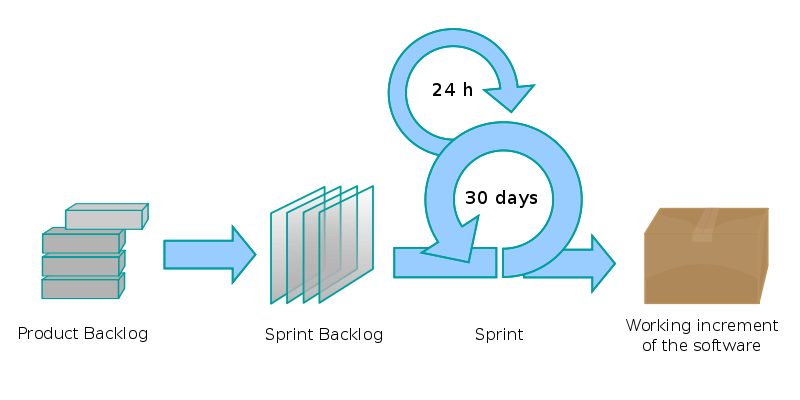
\includegraphics[width=4in]{image/Scrum_process.png}
\caption{Scrum Process}
\label{figure:devchart}
\end{figure}


The Roles: 
\begin{itemize}

\item The Scrum master, who is responsible for leading the process and to enforce the Scrum rules onto the team. He has to make sure that the development team does not overestimate what they can handle during one sprint. He leads the scrum meetings and enlightens and handles obstacles that may appear. 

\item The product owner, represents the stakeholders and is the voice of the customer.

\item The development team, is responsible for delivering potentially shippable product increments at the end of each Sprint. A development team is made up of 3–9 people with cross-functional skills.

\end{itemize}

The Sprints:
\begin{itemize}

\item Normally last from 7 to 30 days .
\item Starts with a planning meeting, where tasks are identified and goals for the sprint is set.
\item Product owner tells the team what tasks should be done in the sprint.
\item The tasks comes from a prioritized list of requirements called the backlog.
\item The team determines what is possible based on this and records this in a sprint backlog.
\item The goals should not be changed during the sprint.

\end{itemize}

The Scrum process is well suited for projects where its difficult to plan too far ahead, where at least some of the aspects of the project are unknown. Its a versatile process which is gives you the ability to handle changes in the requirements and demands from the customer. It allows for the developers to work on different parts of the project at the same time. The design, requirements of the system are not set in stone from the start, and are allowed to evolve during the process. The process delivers unfinished versions at the end of each sprint, which gives the customer a chance to try the system and give continuous feedback to the developers.

The Scrum process is somewhat complex, and it will take time to properly learn and execute the method. You also have to decide on what type of Scrum you are going to use, as there exists multiple forms of Scrum. This can prove to be a time consuming process. And even though the team members know Scrum, they will have to learn the version of scrum decided upon, if it turns out to differ from the one they are used to.
\footnote{\url{http://en.wikipedia.org/wiki/Scrum_(development)}}

\subsubsection{DSDM Atern}
DSDM(Dynamic System Development Method) is an agile software development method, and it was originally meant to provide some discipline to the Rapid Application Development method. The most recent version was launched in 2007 in an effort to make DSDM tool and technique independent, and its called Atern. 

DSDM is an iterative and incremental approach that embraces principles of agile development, including continuous user/customer involvement. It enforces you to deliver incremental versions of the product to the customer, where the main criteria of acceptance is that it meets the current business needs of the customer. It follows the principle that it is always better to deliver something “good enough” early than to deliver everything “perfect” in the end.

DSDM as a method fixes costs, quality and time at the beginning of the project. Through a prioritization method called the “MoSCoW Method”, with musts, shoulds, coulds and won’t haves, it adjusts the scope of the project to meet the given time frame. This allows the development team to focus on the critical functions of the system rather than delivering a perfect system. The method puts a strong focus on actively involving the customer in the development, and continually confirm the solution.

The principle-list of DSDM is quite long and complex. For a team that is not experienced in using the method, the process of learning the method will be time consuming. Also, always having to display the progress to the customer can be time consuming and hinder the development effort. 
Testing is central and shall be done through the whole development process.
\footnote{\url{http://en.wikipedia.org/wiki/DSDM}}

\subsubsection{Extreme Programming}
Extreme programming, hereby referred to as XP, is an agile method designed to reduce cost of changes in requirements by having multiple short development cycles. It includes elements such as pair- programming, extensive code review and unit testing of all the elements of the code. It emphasises frequent communication with the customer and between the developers.

The method embraces changes in the requirements of the project, and it doesn't attempt to define a stable set of requirements at the beginning of the project. In XP a representative for the customer is always available on site to answer any questions the developers might have. It also focuses on frequent releases of working code which serves as checkpoints where the customer can add new requirements.
 
XP puts a lot of focus on the code of the project, the advocates of XP argues that the code is the only truly important product of the system development process. XP as a process does not produce a lot of written documents during the development of the project. In XP programmers are expected to assume a unified client viewpoint and focus on coding rather than documentation of compromise objectives and constraints.
\footnote{\url{http://en.wikipedia.org/wiki/Extreme_Programming}}

\subsection{Conclusion}
If all of the requirements of this project were known in advance and provided by the customer, or the features of the finished product was known and unlikely to change, the waterfall method might be the way to go. But this is a prototype, proof of concept type of project where very little is known about the final product. We were certainly not presented with a finished set of requirements at the beginning of the project, and the requirements we settle on before we start the implementation are also more than likely to change during development. These kind of changes in a waterfall process will be time consuming. Thats why we think that an agile development method will be the best choice for this project.

All of the agile methods described above exhibits properties that will come in useful in this project. They are all based on iterative and incremental development steps, delivering prototypes for the customer to test after each step. This will give the customer a chance to try out unfinished versions of the product and give continuous feedback throughout the project. It can also help the customer to identify new features that they would like to add. They also allows the customer to decide which features to implement in each step, ensuring that the final product will contain the features the customer really need.

The agile methods embrace changes in the requirement and provides ways to handle those changes. They also encourage tight and continuous communication with the customer, which is important to be able to deliver a product that the customer is satisfied with

Of the three methods the group members are most familiar with the Scrum process. The DSDM method is complex and will take a considerable effort to learn and execute correctly. As none of the group members have used DSDM, and we have a limited amount of time in this project, DSDM is of the table. 

XP puts a lot of focus on the code, and delivers a minimal set of documents. We are to write an extensive report about the project, and document every part of it, including compromises and assumptions made. The amount of code in this project will be limited and none of the team members have any experience in working with XP. As a result, XP seems like a bad fit for our project.

The Scrum process does not put as much focus on documentation as the waterfall process, but we think that the amount of documentation produced during the Scrum process will be satisfactory for the report. It will take time to learn how to execute Scrum properly, but since all of the group members are familiar with the basics of process, we think it won’t be too time consuming and worth the effort. The final decision then is to use Scrum as a development method for this project.

\section{Software Testing}

\subsection{Testing Methods}
The purpose of software testing is to uncover software bugs in the system and to document that the system meet the requirements and functionality that was agreed upon for the system. Testing can be implemented at any stage in the development process, traditionally it is performed after the requirements have been defined and the implementation is completed. In agile development processes however, the testing is an ongoing process. The chosen development methodology will in most cases govern the type of testing implemented in a given project.

Software testing methods are traditionally divided into white- and black- box testing. They differ mainly in how the test engineer derives test cases.

\subsubsection{White- Box Testing}
White- box testing focus on the internal structures of a system, and it uses this internal perspective to derive test cases. White- box testing is usually done at unit level, testing specific parts or components of the code. This kind of testing focus on how something is implemented and not necessarily why. Unit testing alone cannot verify the functionality of a piece of software is supposed to exhibit. It can uncover many errors or problems, but it might not detect unimplemented parts of the specification or missing requirements.

\subsubsection{Black- Box Testing}
Black- box testing handles the software as a black- box, meaning it observes the functionality the system exhibits and not the specifics on how it is implemented. The tester only needs to be aware of what the program is supposed to do, he doesn't need to know the specifics on how the functionality is implemented in the code. Black- box testing is typically performed to check if the functionality of the program is according to the agreed upon requirements, both functional and nonfunctional. Black- box testing is usually done at the component, system and release levels of testing.

The main advantage of black- box testing is that no programming knowledge is needed to actually perform the tests. This way you can hire someone outside the development team who has had nothing to do with the implementation of the code to write and perform the tests, and you achieve as little ownership of the code as possible. An argument can be made though that this lack of insight in the specifics of the source code will result in repeated testing of some parts of the code, while other parts could be left untested.

\subsubsection{Test Driven Development}
The principle behind TDD is to develop the code incrementally, along with test for that increment. You don’t move on until the code passes its test. The tests are to be written before you actually implement the new functionality. The process helps programmers clarify their ideas of what a code segment is actually supposed to do. The process is often used in agile development methods.
Benefits from TDD include: 
\begin{itemize}

\item Code coverage, every code segment should be covered at least one test.

\item Regression testing, check to see if changes in the code have not introduced new bugs.

\item Simplified debugging, when a test fails it should be obvious where the problem lies, no need for a debug tool.

\item System documentation, the tests themselves act as a form of documentation that describe what the code should be doing.

\end{itemize}

\subsubsection{Automated Tests}
Automated offers the ability to automatically do regression tests, i.e. testing to uncover if any new code has broken a test that previously passed. If we opt for manual testing regression testing will be very time consuming as every test done so far has to be done over again. With an automated testing framework this job will be a lot easier as you can run a great number of tests in a matter of seconds. Most development languages offers libraries for automated testing.


\subsection{Testing Levels}
Testing can be done at many different levels and in different stages in the development process. Following is the most common partitioning of testing levels and a description on each of them.

\subsubsection{Unit Testing}
Unit testing aims to check specific components, such as methods and objects. Typically you will be testing objects, and you should provide test coverage of all the features of that object. Its important to choose effective unit test cases, that reflect normal operation and they should show that the specific component works. Abnormal inputs should also be included to check if these are processed correctly.

\subsubsection{Component Testing}
Tests bigger components of the system, and their interfaces(communication with other components). Made up of several interacting objects. Component testing is mainly a tool to check if component interfaces behaves according to its specification.

\subsubsection{System Testing}
In a given development project there may be several reusable components that have been developed separately and COTS systems, that has to be integrated with newly developed components. The complete system composing of the different parts is tested at this level. Components developed by different team members or groups may also be integrated and tested at this stage.

\subsubsection{Release Testing}
Release testing is the process of testing a particular release of the system that is intended for use outside of the development team. Often a separate team that has not been involved in the development perform this testing. These kind of tests should focus on finding bugs in the complete system. The objective is to prove to the customer that the product is good enough. This kind of testing could either be based on the requirements of the system or on user scenarios.

\subsubsection{User Testing}
This is a stage in the testing process in which users or customers provide feedback and advice. This could be an informal process where end- users experiment with a new system too see if they like it and that it conforms to their specific needs. Testing on end- users is essential for achieving success in a software process as replicating the exact working environment the system will be used in is difficult to achieve during development. The end users can help provide feedback on how specific functionality will work in an actual work environment.

Another form of user testing involves the customer and its called acceptance testing. Its a process where the customer formally tests a system to decide whether or not it should be accepted, where acceptance implies that payment for the system should be made. Acceptance testing is performed after the release testing phase.

\subsection{Conclusion}
The concept of TDD is to develop exhaustive tests that specify the system, and then writing code with the goal of satisfying the tests. This is useful in systems where the key functionality is in the form of program logic that can be verified to conform to the specification. It is difficult to write such exhaustive tests in applications that rely heavily on GUIs, network connections and database systems because of the added complexity and heterogeneousness that these features involve. In addition, our prototype's exact specifications are likely to change during development, requiring large amounts of test rewriting in the case of TDD, because the tests will be more numerous and because the tests must be more strict. As a result we have opted not to use TDD in this project. We will however be utilizing unit tests with an automated testing framework where it is appropriate and will harvest some of the advantages linked to TDD, like the automated regression testing.

We will be writing unit tests throughout the implementation process and run these continuously. These tests will not be included in the report as test cases. The test cases will rather comprise of component and system tests. Component tests will be used to test specific components and their functionality as well as their interaction with other components. System tests will be used on the system as a whole to check if it meets the agreed upon requirements. These test cases will be derived from the requirements. We will also try include some acceptance tests to include the customer in the testing process. 

We will be utilizing user testing and involve end users to get feedback on the entire system or specific functions. This testing will mainly be used to get feedback on the domain scripting language and how easy it is to understand and use. Preferably it will be done continuously throughout the development process. It is important to involve users as the goal of this project is to ease their workflow. As we are not working with an existing system thats actually in use, there will not exist any real users of this system with experience using it. We will therefore mainly be using our fellow students as test subjects, as they are readily available and technically competent enough to understand the concept and act as superusers. In addition the customer has stated that it will encourage employees from the entire company to us give feedback if we ask for it. Specific solutions can be sent to the customer representative which in turn will relay it to experts on the area it concerns.

\section{Code conventions}
\subsection*{JSLint}
JSLint looks through JavaScript code and detects potentially problematic and unusual syntax in the code to improve the quality of the code. 

JavaScript was originally aimed for web pages with small tasks where the Java platform was too heavy to run and develop for. But JavaScript is capable of much more, and has became used in more and larger projects. However, the lenient and flexible syntax useful for small tasks has proven to make JavaScript troublesome for larger projects. JSLint helps the developer in handling this. \cite{jslint-about}

\subsection*{JSHint}
JSHint is a fork of JSLint which was designed with similar goals of enforcing code quality and avoiding common programming errors, but in a more lenient manner. JSLint is criticized for being a tool that is not first and foremost helpful in preventing bugs or improving readability, but rather a tool that enforces any strict convention as a goal in itself. JSHint attempts to alleviate this, and is more configurable and exhibits less absolutist behaviour. \cite{jshint-about}

\chapter{Requirements}
\section{Usecases/user stories}
\subsection{Planning}
\section{Sequence Diagrams}
\section{Prioritization}
\section{Functional Requirements}
\section{Nonfunctional Requirements}


\section{Test Plan}
This chapter will introduce the overall test plan for this project, and it is based on the IEEE 829 Standard for Software Test Documentation[link to reference]. Some parts of the standard was not deemed to be appropriate for this project and not included as a result. The purpose of this document is to structure the way tests are performed and recorded, assign responsibilities for the testing process as a whole, and to give an outline for the schedule of when the different tests should be performed.

\subsection{Testing Approach}
The testing methods used for this project is discussed in detail in the pre- study. To sum up, we have opted to utilize both black and white box testing in this project. We will write and run unit tests throughout the implementation process together with an automated test framework. The test cases included in the report will be component, system, user and acceptance tests. If additional requirements are added to the system during the Scrum process, new test cases will be created to test the desired functionality.

\subsubsection{Non- Functional Requirements}
The aren’t many non- functional requirements that are essential in this project. It is a proof of concept type of project and the main goal is to prove that the solutions we come up with will get the job done. As a result, tests for common non- functional requirements like performance and security will not be included in the test cases. 

One non- functional requirement worth writing tests for though is usability. The object of the project is to deliver a system that eases the workflow of specific users, and to achieve this we need to develop a system with a large degree of usability. Thats why usability tests will be included in the test cases, in the form of user testing(interviews).

\subsubsection{Testing Process Timeline}
Figure~\ref{figure:testOutline} outlines when the different tests will be performed during the Scrum process. Unit testing will be done throughout the development process in every sprint. Every part of the code implemented should have its own unit tests. Component testing will be done as separate components are finished, typically towards the end of the sprints. Acceptance testing with the customer will be performed in the sprint demo at the end of each sprint. At these demos it will be tested whether the agreed upon functionality for that sprint is actually implemented. System testing will be performed when we have an entire system to test, i.e. when we have implemented some parts of each component needed for the entire system to work. This will likely not be the case until the end of the second sprint. User testing will also be performed in the later sprints, when we have a complete system to present to the test users. Release testing will be performed at the end of the last sprint, to see if the agreed upon functionality for the entire project is indeed present in the system.

\begin{figure}
\centering
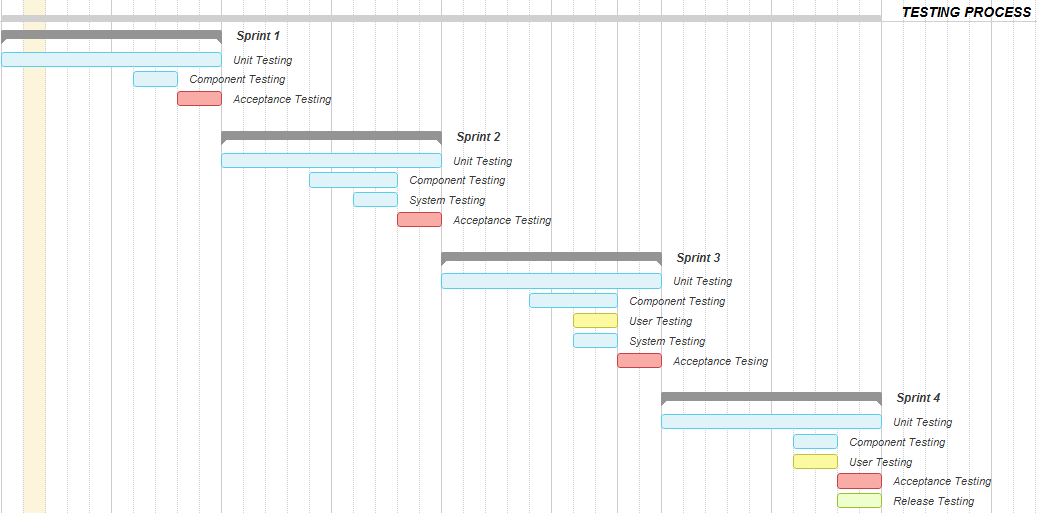
\includegraphics[width=6in]{image/testingProcess.png}
\caption{Testing Process Timeline}
\label{figure:testOutline}
\end{figure}

\subsection{Templates}
The templates stated in Table~\ref{table:testcase} and Table~\ref{table:testreport} will be used to create test cases and to record the results of them.

\begin{table}
\caption{Test Case Template}
\centering
\begin{tabular}{ l l }
\hline
 Item            & Description                                                              \\ 
\hline
 Description     & Description of requirement                                               \\ 
 Tester          & The person responsible for performing the specific test                  \\ 
 Preconditions   & The condition that has to be fulfilled before the execution of this test \\ 
 Feature         & The feature of the system that is to be tested                           \\ 
 Execution steps & Steps to be executed in this test case                                   \\ 
 Expected result & The expected result of the test                                          \\
\hline
\end{tabular}
\label{table:testcase}
\end{table}

\begin{table}
\caption{Test Report Template}
\centering
\begin{tabular}{ l l }
\hline
Item        & Description                             \\ 
\hline
Test ID     & The ID of the given test                \\ 
Description & Description of the requirement          \\ 
Tester      & The person executing the test           \\ 
Date        & The date the test was performed         \\ 
Result      & The result of the test, success or fail. Comment will be added if deemed needed \\
\hline
\end{tabular}
\label{table:testreport}
\end{table}

\subsection{Responsibilities}
The test manager is the one with overall responsibility of the quality of the test plan, and that it will be executed according to the schedule. The person writing test cases and recording test results is responsible for adhering to the templates included in this document.

Each person is responsible for creating unit tests for their own code, and to run these with the automated test framework during development. This will be done to perform continuous testing of the system, and uncover if any new code break some of the previous tests.

We will mainly use someone different to perform the actual test cases than the person who wrote the specific code segment. This is done to achieve as little ownership of the code as possible on part of the tester. But as we are short on manpower and time we can’t guarantee that this is always the case. 

The test cases will be performed towards the end of each sprint when the relevant functionality is implemented. The test will be performed at a time which allows the developers to fix any uncovered bugs in the system before the sprint is ended. 

\subsection{Test Criteria}
A test is considered passed when it achieves the expected result. A test will be considered to have failed if the result of the test differs from the expected one. If we feel a pass/fail of a specific test needs an explanation this will be noted as a comment in the result.
\section{Architecture}
The system is to be described in this chapter. This includes the main parts of the system, the architectural drivers, how they are connected together, and their collaboration. 

The architecture will be described through the 4+1 view model. The party members, or the stakeholders of the system, will have different concerns, so the 4+1 view model will help us describe the system for each of them, and make sure that all expectations are accounted for.  


\subsection{Architectural drivers}
The architectural drivers defines the project and its scope. 
\begin{itemize}{labelitemi}{$\bullet$}
\item Improving the efficiency of the chosen system - The existing system is to improved efficiency vise, so power users will be able to use less time on more tasks. 
\item Proving the concept - Showing that a system can become more efficient through the use of a console. 
\item Modifiability - The system will be constructed for a test concept as a prototype, so further development and maintainability should be made easy for outsiders. It should also be possible to edit the system structure under the process of making it without starting from scratch. 
\item Reach goal from the customer - The customer has a thought of how the system is to look like after we have done our part, we must satisfy these goals and not stray too far from the red thread.  
\end{itemize}


\subsection{Stakeholders}
The stakeholders and their concerns when it comes to the system.

\begin{itemize}{labelitemi}{$\bullet$}
    \item Developer
    \begin{itemize}{labelitemi}{$\bullet$}
        \item Solve the problem and deliver a system the customer will be satisfied with.
        \item Learn new technologies
        \item Get experience with project management
        \end{itemize}
    \item Advisor
    \item Customer
    \begin{itemize}{labelitemi}{$\bullet$}
        \item Gets a working system, which satisfies the customers wants
        \item Get a usable report on the concept, which satisfies the customers wants
    \end{itemize}
    \item End user
    \begin{itemize}{labelitemi}{$\bullet$}
        \item Improve efficiency
        \item Easy to use after some training
    \end{itemize}
\end{itemize}



\subsection{4+1 view model}
The 4+1 view model. Here the views will be described, and how they will look in our architecture. 

\subsubsection{Logical View}
Describes the functionality in the system from the end users perspective.The end users will mainly be power users, wanting to perform object editing tasks efficiently. This view will be described through class, communication and sequence diagram.

The class diagram gives an overview of the class structure of system, and how they collaborate

\begin{figure}
\centering
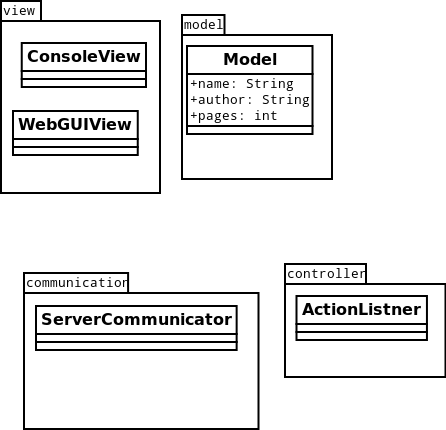
\includegraphics[width=3in]{image/classdiagram.png}
\caption{Class diagram}
\end{figure}

\subsubsection{Development View}
Describes the system from the programmer's perspective. This will be described through how the different component parts are separated. Component and package diagrams will show this.

These components form a three layered structure, and communicate with each other through the neighboring layer

\begin{figure}
\centering
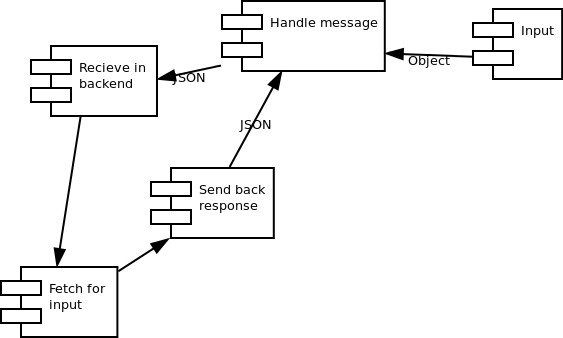
\includegraphics[width=3in]{image/componentdiagram.png}
\caption{Component diagram}
\end{figure}

\subsubsection{Process View}
Describes the dynamic aspect of the system, and explains how the different parts of the system will communicate at runtime. This is described with a activity diagram.

The user will ask for an object from the backend, this will be delivered to the client through the communication channel as a json object, the client will interpret this and the user can then edit it through the console, and send it back to the backend.

\begin{figure}
\centering
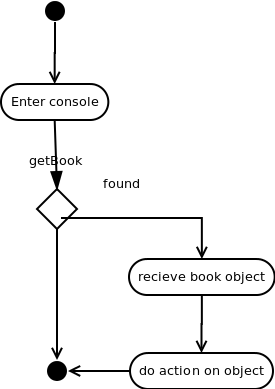
\includegraphics[width=3in]{image/activitydiagram.png}
\caption{Activity diagram}
\end{figure}

\subsubsection{Process View}
Describes the system from the system engineer's perspective. And explains the physical connections between the software components. Described through a deployment diagram. 
With the console the user can fetch the wanted objects from the backend service.

\begin{figure}
\centering
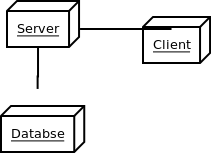
\includegraphics[width=3in]{image/deploymentdiagram.png}
\caption{Deployment diagram}
\end{figure}

%\subsubsection{Scenarios}
%Describes the system through a set of use cases/scenarios. These use cases/scenarios describes how the objects and processes work together.


\subsection{Tactics}
The architectural tactics are used to describe how different qualities of the system are achieved. 

\subsubsection{Modifiability}
Anticipate changes:

Probable changes should be anticipated, and accounted for, so extending the system with new functionality should be possible. This is important since we are dealing with a prototype/proof of concept system. So the customer might change the direction we are going in through out the project, this will lead to changes, and the architecture should be able to bend after these new inputs. 

This can be handled with a well defined functionality map, so that the expected system functionalities are accounted for when the system is constructed. 


\subsection{Architectural patterns}
The patterns can help solve different kinds of problems with know solutions on new problems.

Multi-tier

The architecture of the system will be of the multi-tier kind. This means that the presentation, application processing and data management functions will be separated logically. The application (console) will translate the task of the end user, and 

The console - Translate the task of the end user.
The logical tier - Will receive the translated task from the console, and fetch information from the data storage specified by the console, and set it back to the user.
The data storage - The last tier, and it will contain the information from the library.

figure of the 3 tiers. 

MVC

The client gui and console communication. Since the action made in the console should be reflected in the gui and vice versa, is it natural to use a model-view-controller pattern. The information in the model will then be separated from the view (the display) and the controller which performs an update on the model. 


\subsection{Rationale}

\chapter{Sprint 1}
\section{Planning}
We started the sprint with a sprint planning meeting September 24th. The plan for this sprint is to implement a basic implementation of the system, so that we have something to show the customer at the end of the sprint. We chose user stories from the backlog that would enable us to this, a client and server offering only the most basic operations. 

\subsection{Duration}
This sprint started on September 24th and will last for two weeks. A customer demo will be held at October 04th to show of what we have achieved during the sprint and to ensure that the customer agrees with the implementation.

\subsection{Sprint Goal}
The goal for the first sprint is to get a basic version of the library application working. This includes creating a basic GUI with both the graphical web- application and the console side by side, creating a server capable of storing objects and establish communication between the server and client through a basic REST api. The user should be able to use both the web- application and the console to add a new book to the system and to list the books currently in the system. In addition we decided to implement the real- time messaging from the server to the clients to verify that the solution we chose in the pre- study would be up to the task.

\subsection{User stories}
The user stories we chose to implement in this sprint with their estimated workload is listed in Table~\ref{table:sp1usrstories}. We assume that we have around 170 hours a sprint for working with the actual user stories. The remaining 30 hours will be used for meetings, demonstrations and project management.

Following is some points to discuss the deviations in estimated effort and actual time used.
\begin{itemize}
\item We used more time on implementation than we planned for. We are still getting used to the fact that we have to document everything, usually we just code and hope for the best. Also we had to spend some time setting up technologies on a server and get them running before we started implementing actual functionality.
\item We used less time on design than we planned. Still getting used to designing everything before we code, up front. We plan to do this better the next sprint
\item We used quite a lot of time less on testing than we estimated. We anticipated that we had to use a considerable time to correct bugs and errors during the testing, but all the test cases passed on the first attempt. We anticipated that we had to spend more time on getting all the technologies we had chosen to play together nicely through extensive testing, but it turned out that they were a great fit, and that it wasn't too much work to get them working together in the way we intended.
\item Once we had implemented the functionality of adding new books, the time used to implement D2 and D5 was considerably reduced, as we could resuse much of the code we had created for D1.
\item The PubNub real- time messaging turned out to be easier to implement with Node.js than we expected. 
\item We ended up spending more time on the Scrum planning meeting than we planned for. In addition we didn't work as many hours that we planned for. As a result we had less time available to implement the user stories. Luckily the it turned out that this time was sufficient to finish all the user stories we planned to implement.
\end{itemize}

\begin{table}
\caption{Sprint 1 User Stories}
\centering
\begin{tabular}{ l p{8cm} l l }
\hline 
			&				&\multicolumn{2}{c}{Hours}			\\
 User Story	& Short Description		&Est.		&Act.	                               \\ 
\hline \\ [-2.0ex]
 \bf{A1}     &\bf{Store objects in database}		&\bf{35}		&\bf{44}          \\ 
		  &Design							&8			&6		\\
		  &Implementation					&18			&29		\\
		  &Testing						&5			&4		\\
		  &Documentation					&4			&5		\\

 \bf{A2}     &\bf{Send real- time messages} 		&\bf{20}		&\bf{13}               \\ 
		  &Design							&4			&2		\\
		  &Implementation					&10			&7		\\
		  &Testing						&4			&3		\\
		  &Documentation					&2			&1		\\

 \bf{A3}     &\bf{Access to domain specific object} 	&\bf{25}		&\bf{22}		     \\ 
		  &Design							&10			&5		\\
		  &Implementation					&10			&10		\\
		  &Testing						&3			&3		\\
		  &Documentation					&2			&4		\\

 \bf{G3}     &\bf{Graphical web- application and console}		&\bf{40}		&\bf{38}		     \\ 
		  &Design							&14			&10		\\
		  &Implementation					&18			&21		\\
		  &Testing						&4			&2		\\
		  &Documentation					&4			&5		\\

 \bf{D1}	  &\bf{Add a new book}				&\bf{15}		&\bf{18}		     \\
		  &Design							&3			&2		\\
		  &Implementation					&8			&12		\\
		  &Testing						&2			&2		\\
		  &Documentation					&2			&2		\\

\bf{D2}	  &\bf{Delete a book}				&\bf{15}		&\bf{7}		     \\
		  &Design							&3			&1		\\
		  &Implementation					&8			&4		\\
		  &Testing						&2			&1		\\
		  &Documentation					&2			&1		\\

 \bf{D5}	  &\bf{List all the books in the system}	&\bf{20}		&\bf{9}		     \\
		  &Design							&5			&2		\\
		  &Implementation					&10			&5		\\
		  &Testing						&3			&1		\\
		  &Documentation					&2			&1		\\
\hline 
		  &\bf{Total:}						&\bf{170}		&\bf{151}		\\
\hline
\end{tabular}
\label{table:sp1usrstories}
\end{table}

\begin{table}
\caption{Sprint 1 Workload}
\centering
\begin{tabular}{ l l l }
\hline 
			&\multicolumn{2}{c}{Hours}			\\
 Task		&Est.			&Act.	                               \\ 
\hline \\ [-2.0ex]
Design			&47		&28		\\
Implementation	&82		&88		\\
Testing			&23		&16		\\
Documentation	&18		&19		\\
\hline
\bf{Total}			&\bf{170}	&\bf{151}		\\
\hline
\end{tabular}
\label{table:sp1workload}
\end{table}


\section{Architecture}
This section will handle the architecture we used for this sprint. The architecture will be described through class diagram and component diagram.


\subsection{4+1 view model}
The 4+1 view model. Here the views will be described, and how they will look in our architecture. 

\subsubsection{Logical View}
Describes the functionality in the system from the end users perspective.The end users will mainly be power users, wanting to perform object editing tasks efficiently. This view will be described through class, communication and sequence diagram.

\begin{figure}
\centering
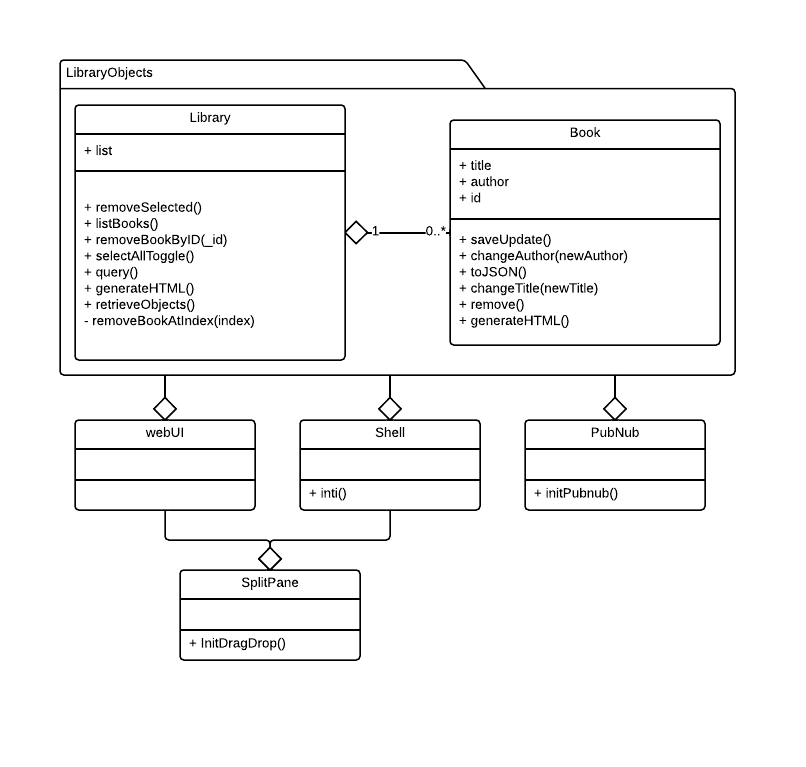
\includegraphics[width=6in]{image/ClassDiagram.png}
\caption{Client Class Diagram}
\label{figure:clientClassDiagram}
\end{figure}

Figure~\ref{figure:clientClassDiagram} The client class diagram gives an overview of the class structure of system, and how they collaborate. We can see that the client consists of two separate views, a GUI and a Shell, which is split by a splitpane so the user can se bouth a GUI interface and the commandline interface. These two views can make changes to the library objects, and get reflected back to the other view. The library objects consists of a library filed with books. The changes done to a book is delivered to other clients and the server through PubNub. 

\begin{figure}
\centering
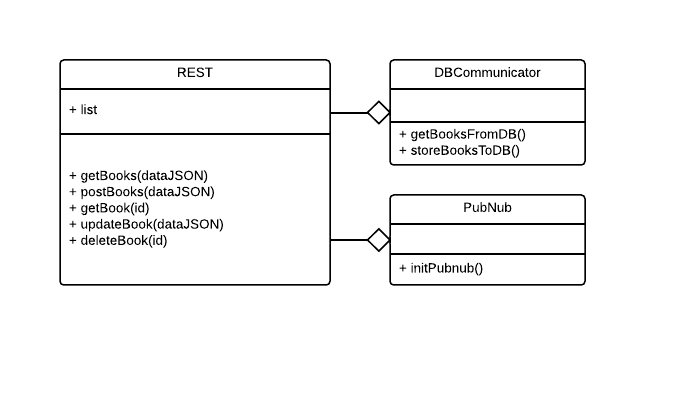
\includegraphics[width=6in]{image/ServerClassDiagram.png}
\caption{Client Class Diagram}
\label{figure:serverClassDiagram}
\end{figure}

Figure~\ref{figure:serverClassDiagram} The server class diagram shows how the REST api is set up, and the communication with the pubnub and db where the library information is stored.


\subsubsection{Development View}
Describes the system from the programmer's perspective. This will be described through how the different component parts are separated. Component and package diagrams will show this.

\begin{figure}
\centering
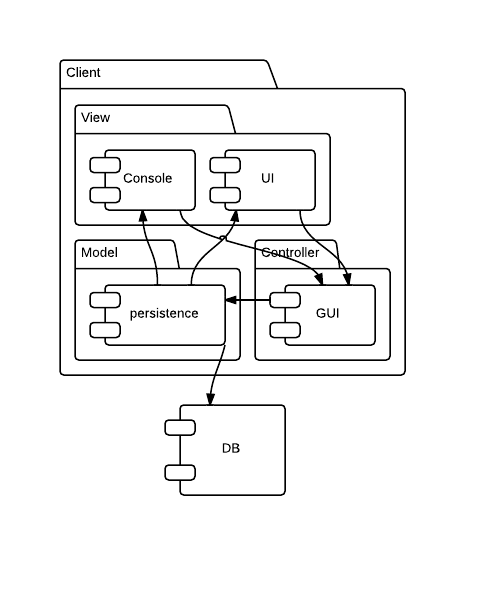
\includegraphics[width=6in]{image/ComponentDiagram.png}
\caption{Component Diagram}
\label{figure:componentDiagram}
\end{figure}

Figure~\ref{figure:componentDiagram} These components form a three layered structure, and communicate with each other through the neighboring layer.



%\subsubsection{Process View}
%Describes the dynamic aspect of the system, and explains how the different parts of the system will communicate at runtime. This is described with a activity diagram.

%The user will ask for an object from the backend, this will be delivered to the client through the communication channel as a json object, the client will interpret this and the user can then edit it through the console, and send it back to the backend.



\subsubsection{Physical View}
Describes the system from the system engineer's perspective. And explains the physical connections between the software components. Described through a deployment diagram. 

\begin{figure}
\centering
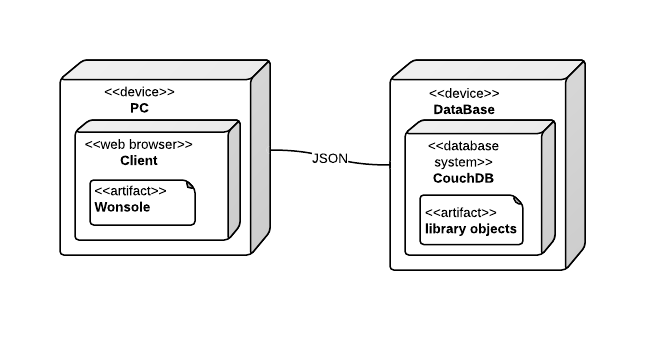
\includegraphics[width=6in]{image/DeploymentDiagram.png}
\caption{Deployment Diagram}
\label{figure:deploymentDiagram}
\end{figure}

Figure~\ref{figure:deploymentDiagram} The structure of the four different parts of the system.


\section{Implementation}

\subsection{RESTful API}
We decided to expose the contents of the database on the central server to the clients through a RESTful API that is served over HTTP. REST is an abbreviation for REpresentational State Transfer, and it basically allows you to get information and perform action equipped only with URLs and standard HTTP methods like GET and POST. The point of REST is having one standard interface for any service. Instead of exposing an interface which has methods, you only expose 4 methods; create, update, read and delete.  You use the URL to describe what object you are performing the action on.

Below each resource is explained in detail, in addition example code with jQuery(JavaScript) will be supplied.

\subsubsection{Base URL}
The base URL for REST API is: http://netlight.dlouho.net:9004/api/

\subsubsection{Get a list of all books}
Description: Returns a list of all the books currently stored in the system 		\\
\newline
Resource URL: http://netlight.dlouho.net:9004/api/books	\\
HTTP Methods: GET		\\
Response format: json	\\
Parameters: None		\\
\newline
Request Example:		\\
GET			http://netlight.dlouho.net:9004/api/books 	\\
\newline
Response:
\begin{verbatim}
[
    {
        "_id": "506b6445b107d7567a000001",
        "author": "An author",
        "title": "Book1"
    },
    {
        "_id": "506c91a1b107d7567a000004",
        "author": "Another author",
        "title": "Book2"
    }
]
\end{verbatim}
Example call in jQuery:
\begin{verbatim}
$.get(‘http://netlight.dlouho.net:9004/api/books’, function(response){
	//Callback function
});
\end{verbatim}

\subsubsection{Add a book to the database}
Description: Adds a book to the database with the supplied parameters. The created book object with a text identifier is returned as a repsonse. 		\\
\newline
Resource URL: http://netlight.dlouho.net:9004/api/books	\\
HTTP Methods: POST		\\
Response format: json	\\
Parameters: None		\\
\newline
Data:
\begin{itemize}

\item title(required): The title of the book that is to be added. Example values: "Title", "A Book".

\item author(required):The author of the book that is to be added. Example values: "Author", "Another Author".

\end{itemize}
Request Example:		\\
POST		http://netlight.dlouho.net:9004/api/books	\\
POST Data	title="Title", author="Author"
\newline
Response:
\begin{verbatim}
[
    {
        "_id": "506b6445b107d7567a000001",
        "author": "Author",
        "title": "Title"
    }
]
\end{verbatim}
Example call in jQuery:
\begin{verbatim}
$.ajax({
  type: 'POST',
  url: ‘http://netlight.dlouho.net:9004/api/books’,
  data: { author:”Author”, title: “Title”},
  success: function(response){
  	//Add book to local storage
  },
  dataType: ‘json’
});
\end{verbatim}

\subsubsection{Get a single book by id}
Description: Returns a single book, specieifed by the id parameter		\\
\newline
Resource URL: http://netlight.dlouho.net:9004/api/books/:id	\\
HTTP Methods: GET		\\
Response format: json	\\
\newline
Parameters: 
\begin{itemize}

\item id(required): This is a text identifier which is used to identify the book in the database. This is created by the database on insertion, and returned to the user. Example value: "506b6445b107d7567a000001"

\end{itemize}
Request Example:		\\
GET		http://netlight.dlouho.net:9004/api/books/506b6445b107d7567a000001	\\
\newline
Response:
\begin{verbatim}
[
    {
        "_id": "506b6445b107d7567a000001",
        "author": "Author",
        "title": "Title"
     }
]
\end{verbatim}
Example call in jQuery:
\begin{verbatim}
$.get(‘http://netlight.dlouho.net:9004/api/books/506b6445b107d7567a000001’, function(response){
	//Callback function
});
\end{verbatim}


\subsubsection{Update a single book by id}
Description: Updates a book with the new values, specified by the supplied id parameter. Returns the updated book object.	\\
\newline
Resource URL: http://netlight.dlouho.net:9004/api/books/:id	\\
HTTP Methods: PUT		\\
Response format: json	\\
Data format: json		\\
Parameters: 			\\
\begin{itemize}

\item id(required): This is a text identifier which is used to identify the book in the database. This is created by the database on insertion, and returned to the user. Example value: "506b6445b107d7567a000001"

\end{itemize}
Data:
\begin{itemize}

\item title(required): The title of the book that is to be added. Example values: "Title", "A Book".

\item author(required):The author of the book that is to be added. Example values: "Author", "Another Author".

\end{itemize}
Request Example:		\\
PUT 		http://netlight.dlouho.net:9004/api/books/506b6445b107d7567a000001	\\
PUT Data: title="NewTitle", author="NewAuthor"
\newline
Response:
\begin{verbatim}
[
    {
        "_id": "506b6445b107d7567a000001",
        "author": "NewAuthor",
        "title": "NewTitle"
     }
]
\end{verbatim}
Example call in jQuery:
\begin{verbatim}
$.ajax({
  type: 'PUT',
  url: ‘http://netlight.dlouho.net:9004/api/books/506b6445b107d7567a000001’,
  data: { author:”NewAuthor”, title: “NewTitle”},
  success: function(response){
  	//Change book attributes in local storage
  },
  dataType: ‘json’
});
\end{verbatim}

\subsubsection{Delete a book by id}
Description: Deletes a book, specified by the supplied id parameter.	\\
\newline
Resource URL: http://netlight.dlouho.net:9004/api/books/:id 	\\
HTTP Methods: DELETE		\\
Parameters: 			
\begin{itemize}

\item id(required): This is a text identifier which is used to identify the book in the database. This is created by the database on insertion, and returned to the user. Example value: "506b6445b107d7567a000001"

\end{itemize}
Request Example:		\\
DELETE	http://netlight.dlouho.net:9004/api/books/506b6445b107d7567a000001	\\
\newline
Example call in jQuery:
\begin{verbatim}
$.ajax({
  type: 'DELETE',
  url: ‘http://netlight.dlouho.net:9004/api/books/5069868335f41ce71a000001’, 
  success: function(response){
  
  },
  dataType: ’json’
});
\end{verbatim}



\subsection{Client-side application}

See Figure~\ref{figure:Wonsole-Sprint1}.

\begin{figure}
\centering
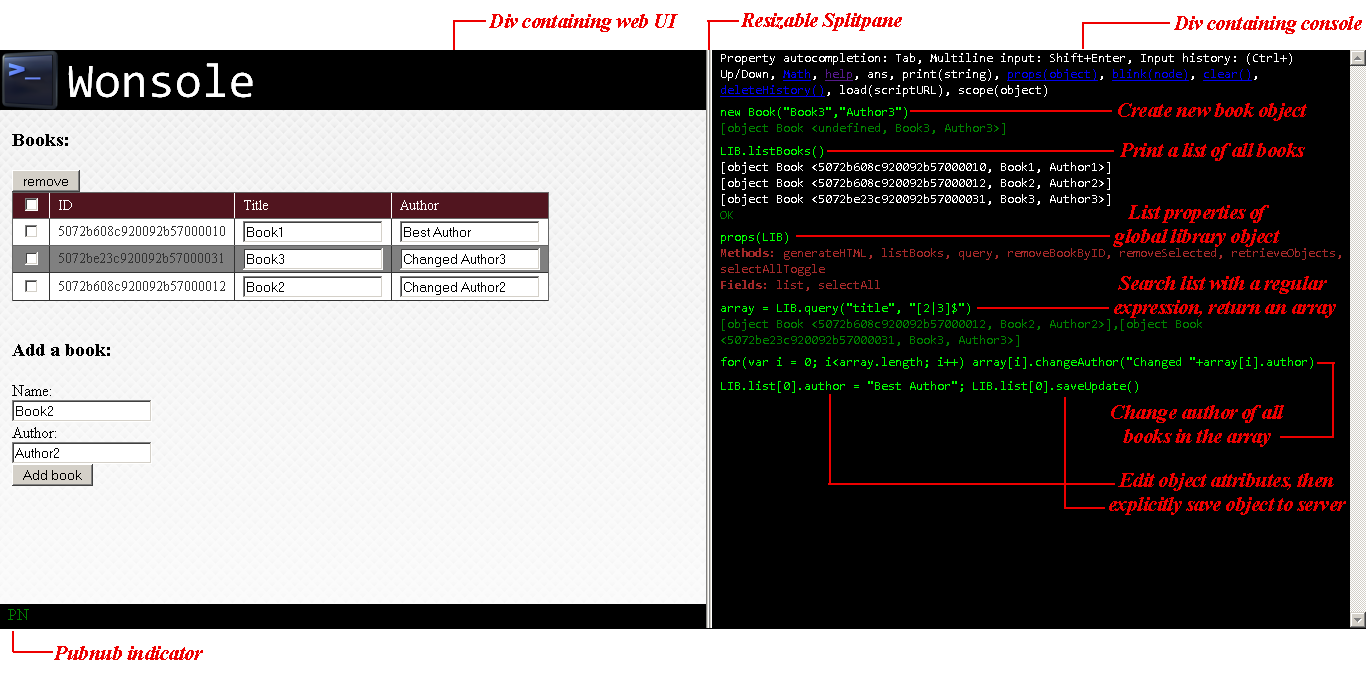
\includegraphics[width=6in]{image/Wonsole-Sprint1.png}
\caption{Wonsole, Sprint 1}
\label{figure:Wonsole-Sprint1}
\end{figure}

\subsubsection{Web UI}
The web user interface is a standard HTML/CSS web site. Lists of objects and their information are generated through JavaScript, and UI elements are associated with JavaScript methods to perform changes to the underlying objects.

\subsubsection{JavaScript Console}
For the console part of the UI, we decided to build off of an existing implementation. We used JavaScript Shell 1.4, which is a command-line interface for JavaScript and DOM. The console will be rather heavily modified to suit the needs of our project. The console current supports a number of useful features, such as listing the variables and methods of an object, suggestions, and a command history. In later sprints, we intend to implement more useful autocompletion, easier navigation of lists of objects as well as better visualization of objects and better integration with the web UI.

The JavaScript Shell is GPL/LGPL/MPL tri-licensed. 
\footnote{\url{http://www.squarefree.com/shell/}}

In the console, it is possible to execute arbitrary JavaScript code. The intended usage is to perform operations on the system's objects only. To implement this particular solution, it must be possible to access all the relevant data through JavaScript objects, and the objects should have appropriate methods to manipulate and store the data. Preferably, the it should also be possible to alter the contents of the web UI by altering the data in the JavaScript objects.

\subsubsection{JavaScript Objects}
We are providing a global object containing a list of books, called LIB, which is a monolith instance of the type Library. The full list of books is retrieved and kept updated from the server. For systems with large data sets, it would be possible to implement caching and more selective loading of server data, but this is not directly interesting to our project. 

Library object specification:
\begin{verbatim}
    function removeSelected ()
    remove all books that are selected in the visible list, will update the web UI and db.
    
    function listBooks()
    List all books into the console.
    
    function removeBookByID(_id)
    Remove a book with the given ID. Will update the web UI and db.

    function selectAllToggle()
    Toggle select all books currently in the visible list. Will update the web UI and db.
    This function is coupled with the checkbox for selecting all books in the list.
    
    function query(parameter1, value1, parameter2, value2 ...)
    Queries the list of books for an array of books where the 
    specified book parameters match their respective values.
    May be called with an arbitrary even number of arguments. 
    The values will be interpreted as regular expressions if they are strings.

    function generateHTML()
    Generate list elements for all books in the system, 
    at the "BOOKTABLE" element in the HTML document.
    
    function retrieveObjects()
    This function retrieves all objects from the server and updates the web UI and db. 
    Will lock the UI until objects have been received.

\end{verbatim}


The aforementioned list contains objects of the type Book. These objects contain information about the book, as well as methods to manipulate their data. Using these methods will also lead to the database and web UI to be updated.

Book object specification:
\begin{verbatim}
    function Book(title, author, id)
    Constructor for the Book object. Will add it to the list of Books in LIB. 
    Should be used with the new keyword.
    If id is null, the object will be sent to the server, and the id will be returned. 
    This will block the UI and then update it.
    Leaving out the id parameter entirely will be interpreted as the id being null.
    id should be null when using this from the console or web UI, 
    but defined in the callback function for retrieving Books.
    
    function saveUpdate()
    Update the book on the server, blocking/unblocking and updating the UI in the process.
    Should be called after altering the Book object's variables.
    
    function changeAuthor(newAuthor)
    Change the author of the book. Will update the web UI and db.
    
    function toJSON()
    Generate a JSON object from this Book.

    function changeTitle(newTitle)
    Change the name of the book. Will update the web UI and db.

    function toggleSelect()
    Toggle whether this book is selected. 
    Will make sure the value of the Book's checkbox is correct, if it exists.
    
    Remove this book from the system. Will update database and UI.
    function remove()

    function generateHTML()
    Generate HTML element(s) for this book. Will not manipulate the UI by itself.
    Returns the DOM HTML element. Should be a table row. Row style will be overridden.
\end{verbatim}


\subsubsection{Pubnub}
Pubnub, previously described in the prestudy, was used to transmit a message to all connected clients when data has been changed. For the first sprint, the client dispatches the message to all other clients when it changes a piece of data, and any client must reload the data from the server when receiving such a message. We realize this is a less-than-optimal and not very tidy solution, so it is likely to be improved in later sprints if it proves to be helpful for the project goal.

\subsubsection{Simulated synchronous behaviour}
For the first sprint, we decided to block user input while the system is communicating with the server, as a quick and safe way to ensure consistency.

jquery.blockUI is a Javascript library we used to achieve this. The intended usage is to simulate synchronous behaviour with AJAX(when necessary) without locking the browser, which is generally unwanted behaviour.
\footnote{\url{http://malsup.com/jquery/block/\#overview}}

\subsubsection{Persistent command history}
The console features a command history that is persistent across page changes, for convenience. PersistJS was used to achieve this.

PersistJS is a JavaScript library which handles client-side storage. It attempts to use the most efficient solution available in the browser, and abstracts away the limitations of certain solutions(such as the size limit on cookies).
PersistJS is under a MIT license.
\footnote{\url{http://pablotron.org/software/persist-js/}}

\subsubsection{Splitpane}
The splitpane is used to let the user customize how much of the window to use for the console and the Web UI. This has been made persistent across page changes.
The splitpane was created by following a drag and drop tutorial by Luke Breuer.
\footnote{\url{http://luke.breuer.com/tutorial/javascript-drag-and-drop-tutorial.aspx}}



\section{Testing}
This section will present the tests performed during the first sprint and thier result

\subsection{Test Results}
We performed a total of 10 test cases during this sprint; TID01-10. The results are listed in Table~\ref{sp1testresults}. The test cases themselves can be found in appendix(TBA).

\begin{table}
\caption{Sprint 1 Test Results}
\centering
\begin{tabular}{ l p{13cm} }

\hline 
Item			&Description		\\
\hline \\ [-2.0ex]

\bf{TestID}		&\bf{TID01}			\\
Description	&Storing objects in a database on the central server	\\
Tester		&Øystein Heimark	\\
Date			&04/10 - 2012	\\
Result		&Success				\\
\hline \\ [-2.0ex]

\bf{TestID}		&\bf{TID02}			\\
Description	&Retrieving objects from the database on the central server	\\
Tester		&Øystein Heimark	\\
Date			&04/10 - 2012	\\
Result		&Success			\\
\hline \\ [-2.0ex]

\bf{TestID}		&\bf{TID03}			\\
Description	&Sending real- time messages from server to client	\\
Tester		&Øystein Heimark	\\
Date			&04/10 - 2012	\\
Result		&Success				\\
\hline \\ [-2.0ex]

\bf{TestID}		&\bf{TID04}			\\
Description	&Alerting clients that there has been added a book to the central database on the server	\\
Tester		&Øystein Heimark	\\
Date			&04/10 - 2012	\\
Result		&Success				\\
\hline \\ [-2.0ex]

\bf{TestID}		&\bf{TID05}			\\
Description	&Verifying that domain specific objects are available through the console	\\
Tester		&Øystein Heimark	\\
Date			&04/10 - 2012	\\
Result		&Success				\\
\hline \\ [-2.0ex]

\bf{TestID}		&\bf{TID06}			\\
Description	&Verifying that there is a console and a graphical interface present on each page\\
Tester		&Øystein Heimark	\\
Date			&04/10 - 2012	\\
Result		&Success			\\
\hline \\ [-2.0ex]

\bf{TestID}		&\bf{TID07}			\\
Description	&Adding a new book to the system with the graphical web- application	\\
Tester		&Øystein Heimark	\\
Date			&04/10 - 2012	\\
Result		&Success			\\
\hline \\ [-2.0ex]

\bf{TestID}		&\bf{TID08}			\\
Description	&Adding a new book to the system with the console	\\
Tester		&Øystein Heimark	\\
Date			&04/10 - 2012	\\
Result		&Success				\\
\hline \\ [-2.0ex]

\bf{TestID}		&\bf{TID09}			\\
Description	&Listing all the books currently in the system using the graphical web- application	\\
Tester		&Øystein Heimark	\\
Date			&04/10 - 2012	\\
Result		&Success				\\
\hline \\ [-2.0ex]

\bf{TestID}		&\bf{TID10}			\\
Description	&Listing all the books currently in the system using the console	\\
Tester		&Øystein Heimark	\\
Date			&04/10 - 2012	\\
Result		&Success			\\
\hline
\end{tabular}
\label{table:sp1testresults}
\end{table}

\subsection{Test Evaluation}
All our tests passed on the first attempt, without any comlications to speak of. The likely cause of this is that we chose to implement a basic protoype for this sprint, with basic functionality all around. There weren't many comlicated components that had to be implemented, and the interfaces between the components were also pretty straight forward. The fact that we performed all of the tests towards the end of the sprint, when all the different components were completed, may also have been a contributing factor. In doing this we avoided getting errors and failed tests because some components were yet to be implemented.

\section{Customer Feedback}


\section{Evaluation}
\subsection{Review}
\subsection{Positive}

\begin{itemize}
\item We delivered a functional system for the demo, with all the promised functionality.
\item The customer was happy with the product and our progress so far.
\item We finished all the user stories, and even additional ones we didn't plan for
\item We divided the work amongst the group members in a good way
\item Conducted a good planning meeting on the first Monday, and we got the customer included in the prioritization of user stories.
\item We received valuable feedback from customer on the demonstration.
\end{itemize}

\subsection{Negative}
\begin{itemize}
\item We didn't do a lot of design up front, and ended up using more time on implementation than we planned for.
\item We weren't good enough to document our work in the report during the sprint. This lead to some work that had to be done after the sprint was finished.
\item We are not using the time tracking system properly at the moment. As a result the documentation of work hours was more time consuming than necessary.
\item Problems with the burndown chart
\item We failed to use the scrum process properly, as we didn't divide the user stories into tasks, and weren't good enough to facilitate daily scrum meetings.
\end{itemize}

\subsection{Planned Responses}
\begin{itemize}
\item Do more design up front, before we start to implemen
\item Break down the user stories into smaller tasks, so its easier to estimate the workload and assign them to different persons.
\item Facilitate the daily Scrum meetings
\item Do more documentation during the sprint, to avoid extra work after the sprint is finished.
\item Fix the burndown chart plugin, and start using it as a tool in the development process
\item Try to log our work hours more accurate, to make it easier to document them afterwards
\end{itemize}

\chapter{Sprint 2}

\minitoc

\subsubsection{Purpose}

This chapter will outline the work we did in the second sprint. It explains in detail how we planned the sprint, including which user stories we chose and the architecture we employed to implement these. Details on the implementation on each user story is also included, as well documentation on the testing process. Finally our evaluation of the second sprint is presented. 

\clearpage

\section{Planning}

\subsection{Duration}
This sprint started on October 8th and lasted for two weeks. A customer demo was held at October 18th to show of what we have achieved during the sprint and to ensure that the customer agreed with the solutions and the direction we were going in.

\subsection{Sprint Goal}
The goal of the second sprint was to increase the functionality of the console. We tried to include user stories that would add functionality that was easy to use and valuable for the end user. The user stories concerned with domain specifics of the system, like implementing support for adding users to the library, will be left untouched in this sprint.

\subsection{Product Backlog} 
Between Sprint 1 and Sprint 2, the customer expressed a desire to improve the usability of the application, by adding features such as auto-completion, tabbing through objects, and better integration between the console and GUI. It was not desired that we implement any more domain-specific functionality. In addition, we decided to alter the backend to support arbitrary objects so that it would not be necessary to change the backend code when creating new types of objects in the application. 

The user stories completed in Sprint 1 were removed, and the following user stories were added:

\begin{itemize}
  \item [\textbf{A4}] As a developer, I want to have a schemaless database, so I don't have to change any code every time the objects change.
  \item [\textbf{G4a}] - As a user, I want commands issued in console to update information in graphical UI.
  \item [\textbf{G4b}] - As a user, I want the actions in graphical UI to print corresponding commands to console.
  \item [\textbf{G9}] As a user, I want the system to be able to autocomplete the commands, and display a list of the available commands on a given object that can be chosen.
  \item [\textbf{G10}] As a user, I want the graphical user interface to indicate which object or group of object I’m working on.
  \item [\textbf{G10a}] - A newly created object should also be highlighted in the user interface.
  \item [\textbf{G11}] As a user, I want the console to be able to cycle through objects in an array one at the time, and for the currently selected object to be displayed on the gui.
  \item [\textbf{G12}] As a user, I want the system to show me details of a record, after I click on a record.
  \item [\textbf{G13}] As a user, I want the system to highlight the changes my by other users, while I work with the system.
  \item [\textbf{G14}] As a user I want to be able to maintain an uninterrupted workflow in the web UI when changes are performed by other users.
  \item [\textbf{G15}] As a user I want to be able to sort the items or find an item, so that i can work with the data effectively
\end{itemize}

The full product backlog for sprint 2 can be found in section \ref{sprint2pb} in the appendix.

\subsection{Sprint Backlog}
The user stories we chose to include in the sprint backlog with their estimated workload is listed in Table~\ref{table:sp2backlog}. As of this sprint we tried to split each user story in the sprint backlog into smaller sub- tasks that could be distributed easily amonst the group members. Each estimate for the subtasks includes design and implementation of the solution. Testing includes writing unit tests as we code, write test cases and to perform them. Documentation includes all the work necessary to document our work on that user story in the report. For this sprint we had 110 hours available for the sprint, exluding work on the report, project management, sprint planning and evaluation. Its a bit less than normal as we decided to put in some extra work on the pre- delivery of the report on October 14th.
\newline
\newline
The decision to make smaller sub- tasks turned out to be succesful, as we were able to estimate the workload more precisly than we did in the last sprint. The tasks were much more detailed as well, instead of general tasks such as "Design" and "Implementation". We experienced that it was easier to estimate the tasks when they represented something concise, and to achieve this they needed to be small enough.
\newline
\newline
There is still room for improvement, as the estimates on some of the sub- tasks were somewhat far away from the actual time used. The tasks that we felt were the most difficult to estimate were the bigger ones. We generally spent less time than planned on these, and we feel that the reason for this was that we failed to break these down to small enough packages. Our general feeling is that the smaller and more concise the tasks are, the better we are able to estimate them. For the next sprint we should make an effort to do more of the same, and try to make the tasks as small and concise as possible and avoid big and general ones.
\newline
\newline
We used less time on the user stories than we planned for this sprint, and a big part of this was due to the pre- delivery of the report. We failed to properly estimate the workload of this delivery, and as a result we had less time available for the user stories. Luckily we were able to finish them using with the time available, mostly because some of the tasks were easier to accomplish than we originally thought. However, this may not be the case in the following sprints. Thats why we feel its important to get the estimates even more precise, so we know exactly how much effort its going to take to achieve the goals we set for the sprints. 

\begin{table}
\caption{Sprint 2 Backlog}
\centering
\begin{tabular}{ l p{8cm} l l }
\hline 
			&				&\multicolumn{2}{c}{Hours}			\\
 User Story	& Short Description		&Est.		&Act.	                               \\ 
\hline \\ [-2.0ex]
 \bf{A4}     &\bf{Update to schemaless database}		&\bf{10}		&\bf{11}          \\ 
		  &Change the server implemenation		&4			&5		\\
		  &Update REST API calls					&2			&1.5		\\
		  &Testing							&2			&2.5		\\
		  &Documentation						&2			&2		\\

 \bf{G4b}     &\bf{Reflect actions from the GUI in the console} 		&\bf{11}		&\bf{13.5}               \\ 
		  &Print the commands in the console				&6			&8		\\
		  &Testing									&3			&3.5		\\
		  &Documentation								&2			&2		\\

 \bf{G9}     &\bf{Autocompletion of commands} 	&\bf{30}		&\bf{22.5}		     \\ 
		  &Add methods to list commands		&4			&2		\\
		  &Create popup menu				&10			&5		\\
		  &Update elements in menu			&4			&3		\\
		  &Make selection of commands possible&3			&3.5		\\
		  &Autocomplete on selection			&1			&1		\\
		  &Testing						&4			&5		\\
		  &Documentation					&4			&3		\\

 \bf{G10}   &\bf{Indicate the selected objects in GUI}		&\bf{26}		&\bf{17}		     \\ 
		  &Design soulution for highlighting elements	&2			&1		\\
		  &Create method for highlighting				&2			&1.5		\\
		  &Create record for selected objects			&4			&2		\\
		  &Respond to changes in selection				&8			&4		\\
		  &Highlight newly created objects				&2			&2		\\
		  &Testing								&4			&3.5		\\
		  &Documentation							&4			&3		\\

 \bf{G11}	  &\bf{Cycle through the current selection}	&\bf{25}		&\bf{18}		     \\
		  &Logic to keep track of selection			&5			&3.5		\\
		  &Update this list when selection changes	&4			&3		\\
		  &Extract objects when cycling through		&7			&4		\\
		  &Update the GUI when selection changes	&2			&2		\\
		  &Testing							&4			&3.5		\\
		  &Documentation						&3			&2		\\

\bf{G12}	  &\bf{Show details on click}			&\bf{8}		&\bf{7.5}		     \\
		  &Make ID clickable					&1			&1		\\
		  &Update relevant section on click		&2			&1.5		\\
		  &Able the user to make changes		&3			&1.5		\\
		  &Testing						&1			&2.5		\\
		  &Documentation					&1			&1		\\
\hline 
		  &\bf{Total:}						&\bf{110}		&\bf{89.5}		\\
\hline
\end{tabular}
\label{table:sp2backlog}
\end{table}


\section{Architecture}
The user stories picked out for sprint two did not have much of an impact on the architecture constructed earlier. We therefore kept using the same architecture as in sprint 1. 

\section{Implementation}

\subsection{Autocomplete}
The autocomplete is made of a jQuery suggestion menu, a modified JavaScript Shell 1.4 and the available objects in the running system. The suggestion menu is attached to the console textarea in Shell. Shell already possessed the ability to generate suggestions based on the user’s input in the console. This information is basically reflected onto the attached suggestion menu, which displays these. Since the system is to be efficient for the selected domain, the available methods and attributes have been cut down, so only the essentials remain, and the user doesn't have to look through unnecessary methods when working.

\subsection{Object highlighting and detailed editing}
It was made possible to click the ID field of book objects in order to highlight their row in the list. This action also filled out the section for adding new books with the information about the given book object. Furthermore, the section for adding new books was enhanced to allow editing of the existing object.

\subsection{Cycling through objects}
Logic was implemented in the console to detect the presence of an array in the user input, and incrementing the index of this array upon pressing the Tab key. The object at the indicated index was then highlighted for editing in the GUI. In order to detect arrays in the textual user input string, the following approach was used:
\begin{itemize}
\item If the string contains the characters '(', ')' or '=', terminate. The code later makes use of the eval() function to determine whether the array is valid, and it was deemed unsafe to risk performing function calls(indicated by the presence of parentheses) or assignment statements(indicated by the presence of an equals sign).
\item Strip complete or partial occurrences of [index] at the end of the string, where 'index' would be an integer literal. Determine the value of 'index' if it is present, set it to 0 otherwise.
\item Evaluate the resulting string and store it in a variable, then test the type of the variable. If the variable is not an array, or if it is an array containing objects that are not book objects, terminate.
\item If the book object at the previously determined index in the array is highlighted in the GUI, increment the index by one, wrapping around if necessary.
\item Add the [index] construct to the end of the string in the console, and highlight the book object at the current index in the array for editing in the GUI.
\end{itemize}

\subsection{Reflection of GUI actions in the console}
The GUI elements were altered so that they sent strings containing JavaScript code to the console for execution, and subsequently displaying the results. 

In itself, the console already contained support for programmatically executing code and displaying the result. However, to make this feasible, some specific implementations had to be altered so as to not use references that were not accessible from the global scope. For instance, the GUI elements for editing book objects were originally implemented by having the book objects create DOM elements with callbacks directly to the book object which created them. This was changed so that the GUI element instead used an index in the global array of books(which was accessible from the console) in order to obtain a reference to the correct book object.

\section{Testing}
This section will present the tests performed during the second sprint and their result.

\subsection{Test Results}
We performed a total of 9 test cases during this sprint; TID11-19. The results are listed in Table~\ref{table:sp2testresults}. The test cases themselves can be found in appendix~\ref{sec:sp2testcases}.

\begin{table}
\caption{Sprint 2 Test Results}
\centering
\begin{tabular}{ l p{13cm} }

\hline 
Item			&Description		\\
\hline \\ [-2.0ex]

\bf{TestID}		&\bf{TID11}			\\
Description	&Storing objects on the server without a schema	\\
Tester		&Øystein Heimark	\\
Date			&19/10 - 2012	\\
Result		&Success				\\
\hline \\ [-2.0ex]

\bf{TestID}		&\bf{TID12}			\\
Description	&Printing commands in the console 	\\
Tester		&Øystein Heimark	\\
Date			&19/10 - 2012	\\
Result		&Success			\\
\hline \\ [-2.0ex]

\bf{TestID}		&\bf{TID13}			\\
Description	&Showing the popup menu	\\
Tester		&Øystein Heimark	\\
Date			&19/10 - 2012	\\
Result		&Failure. The popup menu was displayed, but some of the attributes and methods were missing from the menu				\\
\hline \\ [-2.0ex]

\bf{TestID}		&\bf{TID14}			\\
Description	&Selecting elements from the popup menu	\\
Tester		&Øystein Heimark	\\
Date			&19/10 - 2012	\\
Result		&Success			\\
\hline \\ [-2.0ex]

\bf{TestID}		&\bf{TID15}			\\
Description	&Highlighting selected objects	\\
Tester		&Øystein Heimark	\\
Date			&19/10 - 2012	\\
Result		&Failure. Objects are not automaticly highlighted when they selected from the console. It is however possible to highlight an object from the console using a method call.	\\
\hline \\ [-2.0ex]

\bf{TestID}		&\bf{TID16}			\\
Description	&Highlighting a group of objects\\
Tester		&Øystein Heimark	\\
Date			&19/10 - 2012	\\
Result		&Success			\\
\hline \\ [-2.0ex]

\bf{TestID}		&\bf{TID17}			\\
Description	&Cycling through current selection	\\
Tester		&Øystein Heimark	\\
Date			&19/10 - 2012	\\
Result		&Failure. It is not possible to highlight multiple objects.		\\
\hline \\ [-2.0ex]

\bf{TestID}		&\bf{TID18}			\\
Description	&Highlighting while cycling through objects	\\
Tester		&Øystein Heimark	\\
Date			&19/10 - 2012	\\
Result		&Success	\\
\hline \\ [-2.0ex]

\bf{TestID}		&\bf{TID19}			\\
Description	&Update separate section on clicking a book	\\
Tester		&Øystein Heimark	\\
Date			&19/10 - 2012	\\
Result		&Failure. It is not possible to edit the title of the book in the separate section		\\
\hline

\end{tabular}
\label{table:sp2testresults}
\end{table}

\subsection{Test Evaluation}
Some of our test failed this time. Most of them was due to minor bugs in the system which was easily corrected at once. The remaining failures was due to some missing functionality which was defined by the user stories and where yet to be implemented at the time the testing was performed. However we were able to add this functionality and pass all the tests before the beginning of the third sprint.

\section{Customer Feedback}
This sections covers the feedback we got from the customer, both before and after the sprint.
\newline
\newline
At the beginning of the sprint the customer had a lot of suggestions and opinions on what we should implement in this sprint, and provided us some user stories that he wanted us to implement. He suggested that our focus for this sprint should be on improving the functionality of the console, something the group also wanted to do. 
\newline
\newline
At the end of this sprint the customer was happy with the work we presented, but at the same time felt that the system was still missing something. The workflow was not as fluid as it should be, the console needed a x- factor that appealed to the user an made the console more prominent. The focus should be on adding functionality that adds value to the console. At the moment the console and its features are very programmatic. The customer told us that he would meet with other representatives from the company to talk about the direction they wanted the project to take from this point on, and to maybe find the x- factor we were looking for. We would get this feedback for the start of the third sprint.The customer also requested that we started to test our product on our peers, as feedback from users would be extremly valuable at this point of the project. He suggested that we should devote some time in the next sprint to make and perform the user testing, something the group also felt would be a good idea.

\section{Evaluation}
This section contains the evaluation of the second sprint, and what we plan to improve for the third sprint. The evaluation was performed during an internal meeting with all group members present.

\subsection{Review}

Again we were happy with the product we were able to deliver in the sprint. All the user stories in the sprint backlog were completed, and we feel like we reached the goal of extending the functionality of the console. and think that the features we implemented added great value to the console. Again the customer was happy with the end result, although he felt something was missing. This time the customer was even more included in the planning, and helped us in creating some of the user stories. This allowed them to have a greater influnce on what was to be included in this sprint.
\newline
\newline
We feel like we succeded in addressing some of the issues we faced in the previous sprint regarding our work process. The responses we created after the first sprint turned out to work quite well. Our time logging routines improved significantly, and this eased the work of documenting the workload of each user story. It also helped the team leader to oversee the progress of the sprint and to monitor the work of each of the team members.
\newline
\newline
As mentioned earlier we succeded in creating a more detailed work breakdown structure, and were able to break each user story into smaller tasks. This helped a lot when we estimated the workload of each user story, and made it easier for multiple team members to work on the same user story at once. The distribution of workload was even better than in the first sprint, and a big reason that we were able to finish all the user stories in time.
\newline
\newline
The testing proved to be more useful this time, as we uncovered multiple errors in the system and in some cases some missing functionality in some of the user stories. Although this was great and it showed that the testing surved a purpose, the timing of the testing could be improved. In this sprint we performed the test cases at the end of the sprint, and this resulted in errors discovered after the cusotmer demo. Ideally they should have been discovered and corrected before the demonstration to the customer.
\newline
\newline
Before the sprint we set out to improve the Scrum process, but we only partly succeded. We were able to organize the daily meetings, but we think there is still some improvements to be made here. We also had some technical issues during the demo which made it difficult for us to perform a proper demonstration of the features we had implemented. The technical aspect of the demo should have been prepared better, and we should always have a backup solution in case we experince problems during the demonstration.
\newline
\newline
A big downside to this sprint was the fact that we failed to estimate the workload neccessary for the pre- delivery. This ate up a lot more time than expected and as a result we were left with considerably less time for the implementation than we planned for. We were able to adjust and complete all the user stories, but we were lucky considering some of them turned out to be easier than expected.


\subsubsection{Positive Experiences}
\begin{itemize}
\item Much improved time tracking
\item Better breakdown of the user stories
\item Customer more included in the planning
\item Testing proved useful
\end{itemize}


\subsubsection{Negative Experiences}
\begin{itemize}
\item Can still improve on some parts of the Scrum process
\item Failed to estimate the workload of the pre- delivery
\item Technical issues during demostration
\item Testing performed too late
\end{itemize}

\subsection{Planned Responses}
These are the actions we have planned for the next sprint to improve our work process.

\subsubsection{Testing}
In this sprint we experienced how important the testing process can be in regards to finding errors and bugs we would otherwise fail to discover. However we performed the test cases too late to be able to correct them before the customer demonstration. Thats why we in the next sprint will perform the tests earlier, we will then manage to fix the issues in time.

\subsubsection{Demo}
For the next sprint we should properly prepare for the demo, and make it easier for the customer to follow the workflow. Also we should have a backup solution for how we are going to present our product if we experince technical difficulties again.

\subsubsection{Scrum}
Put even more effort into creating concise user stories and to break these into small tasks which can easily be distributed among the team members. We feel like this was something which contributed to the success of this sprint, and we would like to improve this even further in the next sprint. Also we aim to put more effort into the daily Scrum meetings and utilize these properly.
\chapter{Sprint 3}

\minitoc

\subsubsection{Purpose}

This chapter will outline the work we did in the third sprint. It explains in detail how we planned the sprint, including which user stories we chose and the architecture we employed to implement these. Details on the implementation on each user story is also included, as well documentation on the testing process. Finally our evaluation of the third sprint is presented. 

\clearpage

\section{Planning}

\subsection{Duration}
This sprint started on October 22th and will last for two weeks. A customer demo will be held at 1st of November to show of what we have achieved during the sprint and to ensure that the customer agrees with the solutions and the direction we are going in.

\subsection{Sprint Goal}
The goal for this sprint is to redesign the system to accomodate the new wishes from the customer, and present a working protoype with the suggested technologies.

\subsection{User stories}

\section{Architecture}
\subsection{4+1 view model}
\subsubsection{Logical View}
\subsubsection{Development View}
\subsubsection{Process View}
\subsubsection{Physical View}

\section{Implementation}

\section{Testing}
\subsection{Test Results}
\subsection{Test Evaluation}

\section{Customer Feedback}
This sections covers the feedback we got from the customer, both before and after the sprint.
\newline
\newline
At the end of sprint 2 the customer representative informed us that he would have a meeting with others in the company, to try to identify what our product was missing, a x- factor that would appeal to the users and promote the console.

At the Scrum meeting for the third sprint he announced that they had indeed found this x- factor. He wanted us to return to the roots of the project, namely adding scripting to a web- page. We should focus on adding functionality which is impossible or difficult and time consuming to do in a regular GUI.

He wanted us to add functionality that would show of the advantages of the technologies we are using, and how it would not be possible to do this with more traditional technologies. He listed some general use cases he wanted us to implement, and suggested that we looked into another solution for the backend. This was because he felt that this solution was better suited for the use cases he now presented us. He was aware of the time constraints of the project and did not expect us to manage to implement all the functionality he mentioned. But it was important that we could document that it would be possible to implement it with the technologies we are using in this project.


\section{Evaluation}
\subsection{Review}
\subsection{Positive}
\subsection{Negative}
\subsection{Planned Responses}

\chapter{Sprint 4}
\section{Planning}
\subsection{Duration}
\subsection{Sprint Goal}
\subsection{User stories}
\section{Architecture}
\subsection{4+1 view model}
\subsubsection{Logical View}
\subsubsection{Development View}
\subsubsection{Process View}
\subsubsection{Physical View}
\section{Implementation}
\section{Testing}
\subsection{Test Results}
\subsection{Test Evaluation}
\section{Customer Feedback}
\section{Evaluation}
\subsection{Review}
\subsection{Positive}
\subsection{Negative}
\subsection{Planned Responses}

\chapter{Conclusion}


\chapter{Appendices}
\section{Test Cases}
\subsection{Sprint 1}

\begin{table}
\caption{Test Case TID01}
\centering
\begin{tabular}{ l p{13cm} }
\hline 
 Item            & Description                                                              \\ 
\hline \\ [-2.0ex]
 Description     & Storing objects in a database on the central server                        \\ 
 Tester          & Øystein Heimark                  \\ 
 Preconditions   & There needs to be a server running with a connection to a database available \\ 
 Feature         & Test the ability to store objects permanently on the server from the client  \vspace{3pt}                     \\ 
\hline \\ [-1.5ex]
 Execution steps & \pbox{13cm}{1. Open a new client \\ 2. Call the appropriate method for storing a new object with a given set of attributes from the client. \\ 3. List the content of the database and observe if the new object is indeed stored with its correct attributes. } \vspace{3pt} \\
\hline \\ [-1.5ex]
 Expected result & The object is stored in the database with the correct attributes                                          \\
\hline 
\end{tabular}
\label{table:testcasetid01}
\end{table}


\begin{table}
\caption{Test Case TID02}
\centering
\begin{tabular}{ l p{13cm} }
\hline 
 Item            & Description                                                              \\ 
\hline \\ [-2.0ex]
 Description     & Retrieving objects from the database on the central server \\ 
 Tester          & Øystein Heimark                  \\ 
 Preconditions   & There needs to be a server running with a connection to a database available \\ 
 Feature         & Test the clients ability to retrieve objects from the server   \vspace{3pt}                     \\ 
\hline \\ [-1.5ex]
 Execution steps & \pbox{13cm}{1. Open a new client. \\ 2. Call the appropriate method for retrieving an object. \\ 3. Observe the response from the server. } \vspace{3pt} \\
\hline \\ [-1.5ex]
 Expected result & The object is successfully retrieved from the server with the correct attributes          \\
\hline 
\end{tabular}
\label{table:testcasetid02}
\end{table}


\begin{table}
\caption{Test Case TID03}
\centering
\begin{tabular}{ l p{13cm} }
\hline 
 Item            & Description                                                              \\ 
\hline \\ [-2.0ex]
 Description     & Sending real- time messages from server to client \\ 
 Tester          & Øystein Heimark                  \\ 
 Preconditions   & There needs to be a server able to send messages up and running, and a client ready to receive \\ 
 Feature         & Test the ability to send real- time messages from server to client   \vspace{3pt}                     \\ 
\hline \\ [-1.5ex]
 Execution steps & \pbox{13cm}{1. Open a new client. \\ 2. Send a message from the server with the associated method. \\ 3. Observe the output on the client side. } \vspace{3pt} \\
\hline \\ [-1.5ex]
 Expected result & The message will be received by the client and displayed within one second from when the message is sent from the server.          \\
\hline 
\end{tabular}
\label{table:testcasetid03}
\end{table}

\begin{table}
\caption{Test Case TID04}
\centering
\begin{tabular}{ l p{13cm} }
\hline 
 Item            & Description                                                              \\ 
\hline \\ [-2.0ex]
 Description     & Alerting clients that there has been added a book to the central database on the server \\ 
 Tester          & Øystein Heimark                  \\ 
 Preconditions   & TID03 and either TID05 or TID06 must alredady have passed. The server must be running \\ 
 Feature         &The ability to alert multiple clients that a new book is added to the system real- time \vspace{3pt}                     \\ 
\hline \\ [-1.5ex]
 Execution steps & \pbox{13cm}{1. Open the application with multiple clients. \\ 2. Add a new book from one of the clients. \\ 3. Observe the output on all the clients} \vspace{3pt} \\
\hline \\ [-1.5ex]
 Expected result & All the clients will be alerted within one second that a new book has been added, and the list of books in the client will be updated.          \\
\hline 
\end{tabular}
\label{table:testcasetid04}
\end{table}


\begin{table}
\caption{Test Case TID05}
\centering
\begin{tabular}{ l p{13cm} }
\hline 
 Item            & Description                                                              \\ 
\hline \\ [-2.0ex]
 Description     & Verifying that domain specific objects are available through the console \\ 
 Tester          & Øystein Heimark                  \\ 
 Preconditions   &A console must be available \\ 
 Feature         &The ability to work directly with domain specific objects and objects attributes \vspace{3pt}                     \\ 
\hline \\ [-1.5ex]
 Execution steps & \pbox{13cm}{1. Open a console. \\ 2. Create a book object. \\ 3. Change the attribute of the newly created object by command.} \vspace{3pt} \\
\hline \\ [-1.5ex]
 Expected result & The user is able to retrieve objects and change their attributes via the console.          \\
\hline 
\end{tabular}
\label{table:testcasetid05}
\end{table}


\begin{table}
\caption{Test Case TID06}
\centering
\begin{tabular}{ l p{13cm} }
\hline 
 Item            & Description                                                              \\ 
\hline \\ [-2.0ex]
 Description     & Verifying that there is a console and graphical interface present on each page\\ 
 Tester          & Øystein Heimark                  \\ 
 Preconditions   &None \\ 
 Feature         &Simultaneous display of console and graphical interface \vspace{3pt}                     \\ 
\hline \\ [-1.5ex]
 Execution steps & \pbox{13cm}{1. Open a new instance of the application with a web- client. \\ 2. Observe if there is a graphical interface as well as a console present.} \vspace{3pt} \\
\hline \\ [-1.5ex]
 Expected result & Console and graphical interface is present on the same page.          \\
\hline 
\end{tabular}
\label{table:testcasetid06}
\end{table}


\begin{table}
\caption{Test Case TID07}
\centering
\begin{tabular}{ l p{13cm} }
\hline 
 Item            & Description                                                              \\ 
\hline \\ [-2.0ex]
 Description     & Adding a new book to the system with the graphical web- application \\ 
 Tester          & Øystein Heimark                  \\ 
 Preconditions   & The server with the REST api must be running. A graphical interface must be available. \\ 
 Feature         & The ability to add new books to the system from a client with the graphical web- application   \vspace{3pt}                     \\ 
\hline \\ [-1.5ex]
 Execution steps & \pbox{13cm}{1. Open the application with a web client \\ 2. Add a new book from the web- application on the client. \\ 3. List the books currently on the system and observe if the new book is added.} \vspace{3pt} \\
\hline \\ [-1.5ex]
 Expected result & The new book is added to the system and the list of books with the attributes stated in the creation of the book.          \\
\hline 
\end{tabular}
\label{table:testcasetid07}
\end{table}



\begin{table}
\caption{Test Case TID08}
\centering
\begin{tabular}{ l p{13cm} }
\hline 
 Item            & Description                                                              \\ 
\hline \\ [-2.0ex]
 Description     & Adding a new book to the system with the console. A console must be available \\ 
 Tester          & Øystein Heimark                  \\ 
 Preconditions   & The server with the REST api must be running \\ 
 Feature         & The ability to add new books to the system from a client with the console.   \vspace{3pt}                     \\ 
\hline \\ [-1.5ex]
 Execution steps & \pbox{13cm}{1. Open the application with a web client \\ 2. Add a new book from the console on the client. \\ 3. Observe the list of the books currently on the system and observe if the new book is in this list.} \vspace{3pt} \\
\hline \\ [-1.5ex]
 Expected result & The new book is added to the system and the list of books with the attributes stated in the creation of the book.          \\
\hline 
\end{tabular}
\label{table:testcasetid08}
\end{table}


\begin{table}
\caption{Test Case TID09}
\centering
\begin{tabular}{ l p{13cm} }
\hline 
 Item            & Description                                                              \\ 
\hline \\ [-2.0ex]
 Description     & Listing all the books currently in the system using the graphical web- application \\ 
 Tester          & Øystein Heimark                  \\ 
 Preconditions   & The server with the REST api must be running. There has to be books stored in the database. A graphical interface must be available\\ 
 Feature         & The ability to get an overview of the books currently in the system using the web- application   \vspace{3pt}                     \\ 
\hline \\ [-1.5ex]
 Execution steps & \pbox{13cm}{1. Obtain a list of all the books in the system directly from the central database/server \\ 2. Use the graphical web- application to get a list of all the books in the system \\ 3. Compare the result from step two to the one obtained in step 1, and verify that they contain the same books.} \vspace{3pt} \\
\hline \\ [-1.5ex]
 Expected result & The list of books presented in the graphical web- application is identical to the one stored on the central database/server.          \\
\hline 
\end{tabular}
\label{table:testcasetid09}
\end{table}


\begin{table}
\caption{Test Case TID10}
\centering
\begin{tabular}{ l p{13cm} }
\hline 
 Item            & Description                                                              \\ 
\hline \\ [-2.0ex]
 Description     & Listing all the books currently in the system using the console. \\ 
 Tester          & Øystein Heimark                  \\ 
 Preconditions   & The server with the REST api must be running. There has to be books stored in the database.  A console must be available\\ 
 Feature         & The ability to get an overview of the books currently in the system using console.   \vspace{3pt}                     \\ 
\hline \\ [-1.5ex]
 Execution steps & \pbox{13cm}{1. Obtain a list of all the books in the system directly from the central database/server \\ 2. Use the console to get a list of all the books in the system \\ 3. Compare the result from step two to the one obtained in step 1, and verify that they contain the same books.} \vspace{3pt} \\
\hline \\ [-1.5ex]
 Expected result & The list of books presented in the console is identical to the one stored on the central database/server.          \\
\hline 
\end{tabular}
\label{table:testcasetid10}
\end{table}




It was shown in \cite{example}

\bibliography{references}

\end{document}
